%        File: prelimPres.tex
%     Created: Thu Aug 25 11:00 AM 2011 C
% Last Change: Thu Aug 25 11:00 AM 2011 C
%
%\documentclass[11pt,handout]{beamer}
\documentclass[9pt]{beamer}
\usetheme[white]{Wisconsin}
%\title[short title]{long title}
\title[Integrated Repository Model]{An Integrated Used Fuel Disposition and Generic Repository Model}
%\subtitle[short subtitle]{long subtitle}
\subtitle[CNERG Update]{Update to CNERG Orientation 2012}
%\author[short name]{long name}
\author[K. Huff]{Kathryn D. Huff}
%\date[short date]{long date}
\date[8.30.2012]{August 30, 2012}
%\institution[short name]{long name}
\institute[UW-Madison]{University of Wisconsin-Madison}
% Page numbers.
\setbeamertemplate{footline}[page number]
% Those icons  in the references are terrible looking.
\setbeamertemplate{bibliography item}[text]
% need some error functions? Me too.
\DeclareMathOperator{\erf}{erf}
\DeclareMathOperator{\erfc}{erfc}


\begin{document}
%%%%%%%%%%%%%%%%%%%%%%%%%%%%%%%%%%%%%%%%%%%%%%%%%%%%%%%%%%%%%
%% From uw-beamer Here's a handy bit of code to place at 
%% the beginning of your presentation (after \begin{document}):
\newcommand*{\alphabet}{ABCDEFGHIJKLMNOPQRSTUVWXYZabcdefghijklmnopqrstuvwxyz}
\newlength{\highlightheight}
\newlength{\highlightdepth}
\newlength{\highlightmargin}
\setlength{\highlightmargin}{2pt}
\settoheight{\highlightheight}{\alphabet}
\settodepth{\highlightdepth}{\alphabet}
\addtolength{\highlightheight}{\highlightmargin}
\addtolength{\highlightdepth}{\highlightmargin}
\addtolength{\highlightheight}{\highlightdepth}
\newcommand*{\Highlight}{\rlap{\textcolor{HighlightBackground}{\rule[-\highlightdepth]{\linewidth}{\highlightheight}}}}
%%%%%%%%%%%%%%%%%%%%%%%%%%%%%%%%%%%%%%%%%%%%%%%%%%%%%%%%%%%%%

%||||||||||||||||||||||||||
\AtBeginSection[]
{
   \begin{frame}
       \frametitle{Outline}
       \tableofcontents[currentsection]
   \end{frame}
}

%||||---------------
\frame{
\titlepage
}
%---------------||||


%||||---------------
\frame{
\frametitle{Outline}
\tableofcontents[]
}
%---------------||||
\section{Introduction}
\subsection{Motivation}
% Waste is a problem
% Decisionmakers are contemplating many fuel cycle options
% Decisionmakers are contemplating many repository options
% Interfacing between FCO/SA campaign and UFD campaign

\begin{frame}[ctb!]
  \frametitle{Future Disposal System Options}
   \begin{minipage}{0.44\textwidth}
     \begin{figure}[h!]
         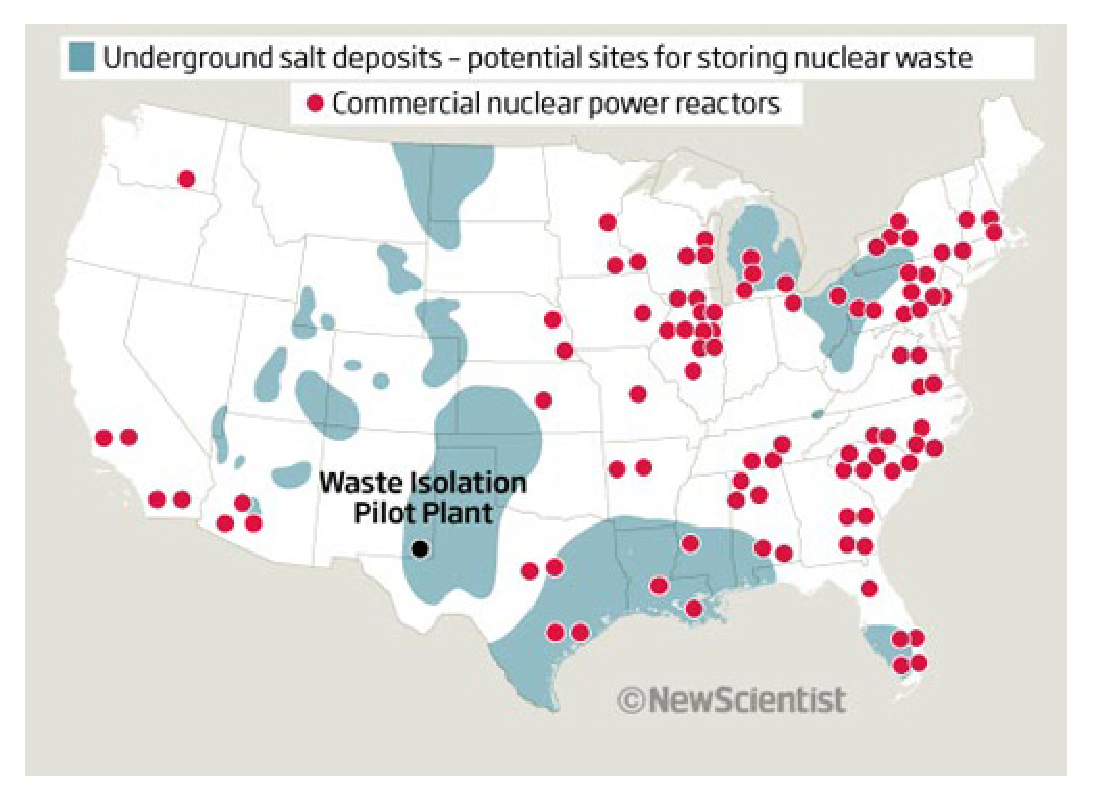
\includegraphics[width=0.8\textwidth]{saltNewScientist.eps}
         \caption{U.S. Salt Deposits ref. \cite{newscientist_where_2011}}
     \end{figure}
     \begin{figure}[h!]
         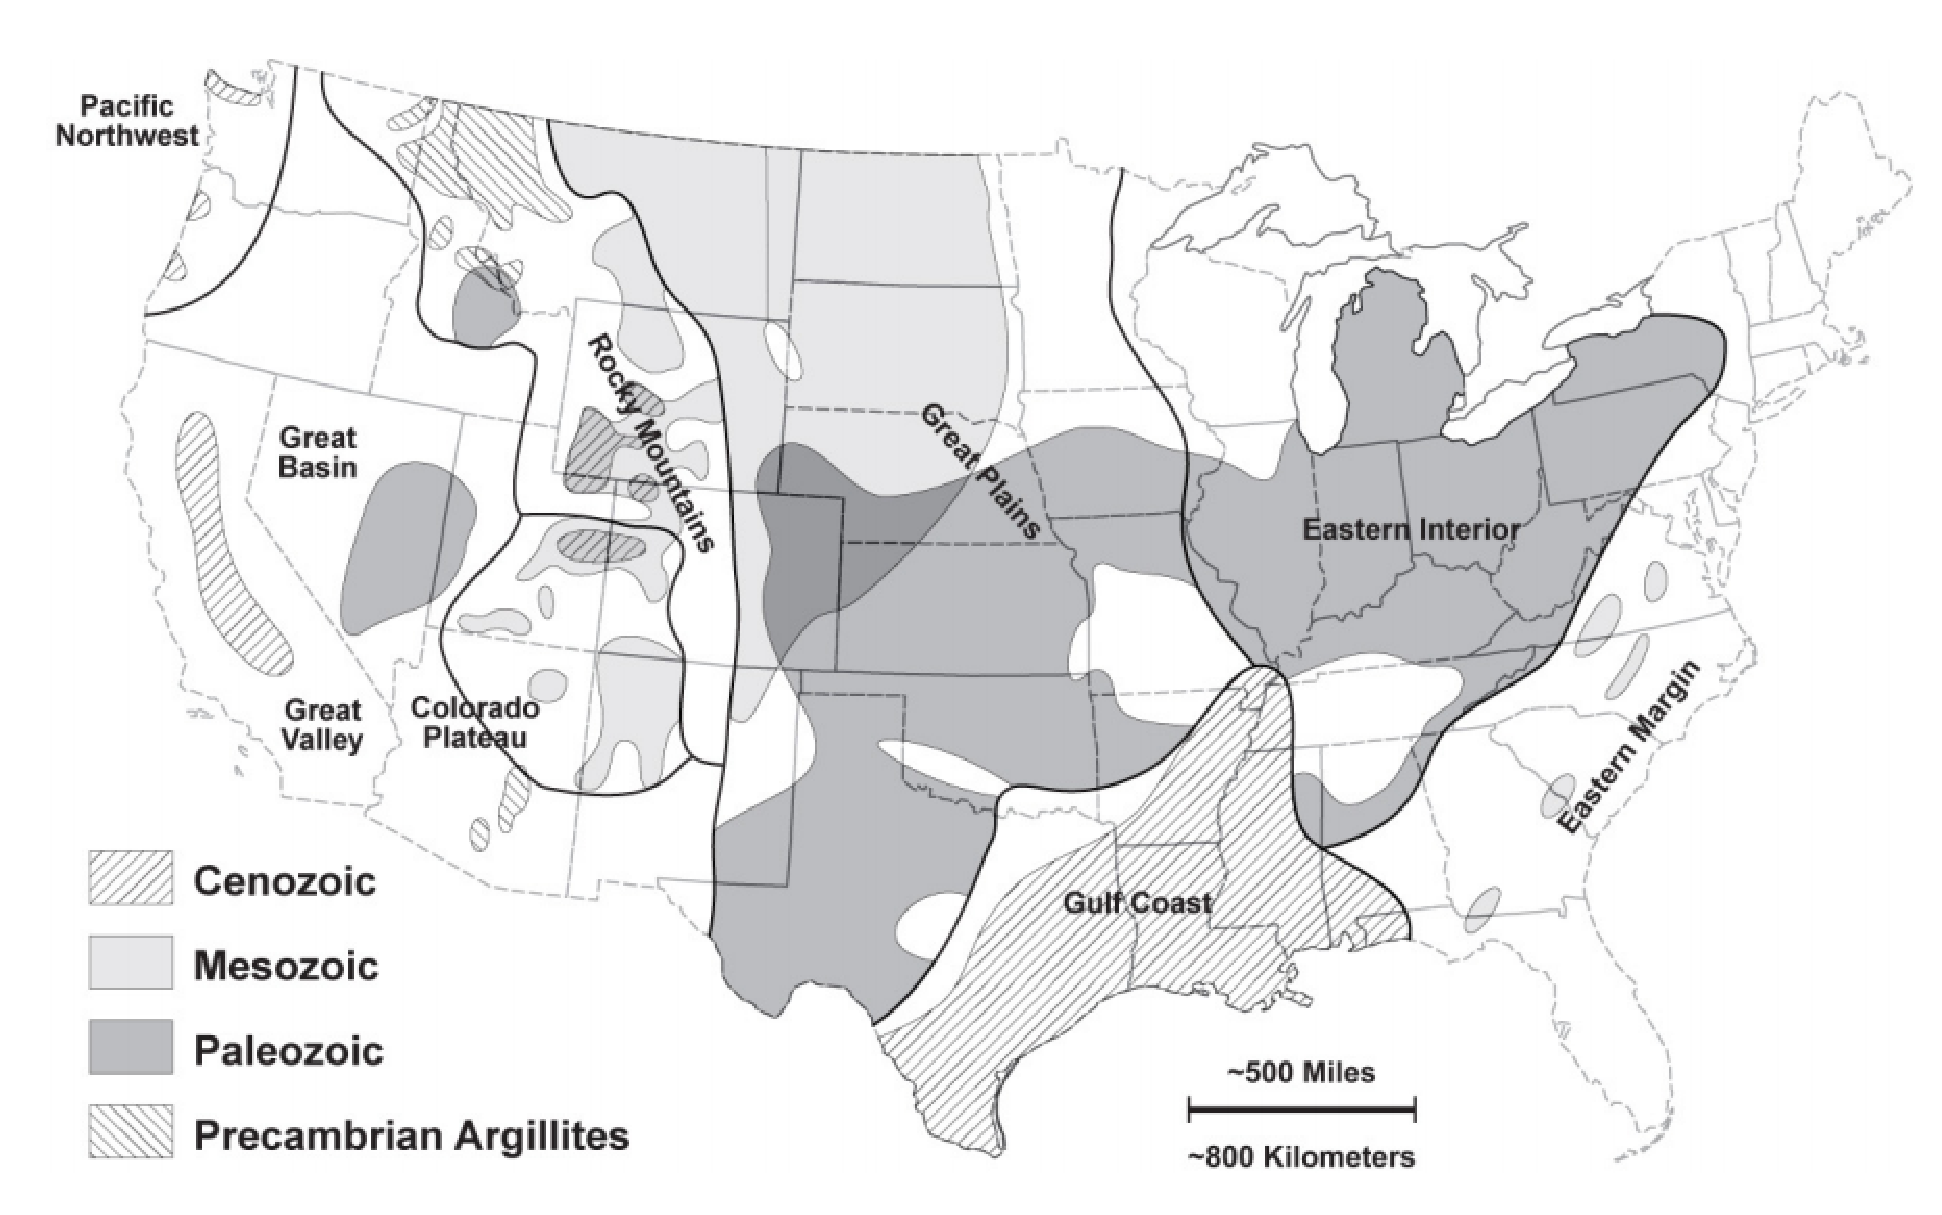
\includegraphics[width=0.8\textwidth]{clayGonzales.eps}
         \caption{U.S. Clay Deposits ref. \cite{gonzales_shales_1985}}
     \end{figure}
   \end{minipage}
   \hspace{0.01cm}
   \begin{minipage}{0.44\textwidth}
     \begin{figure}[h!]
         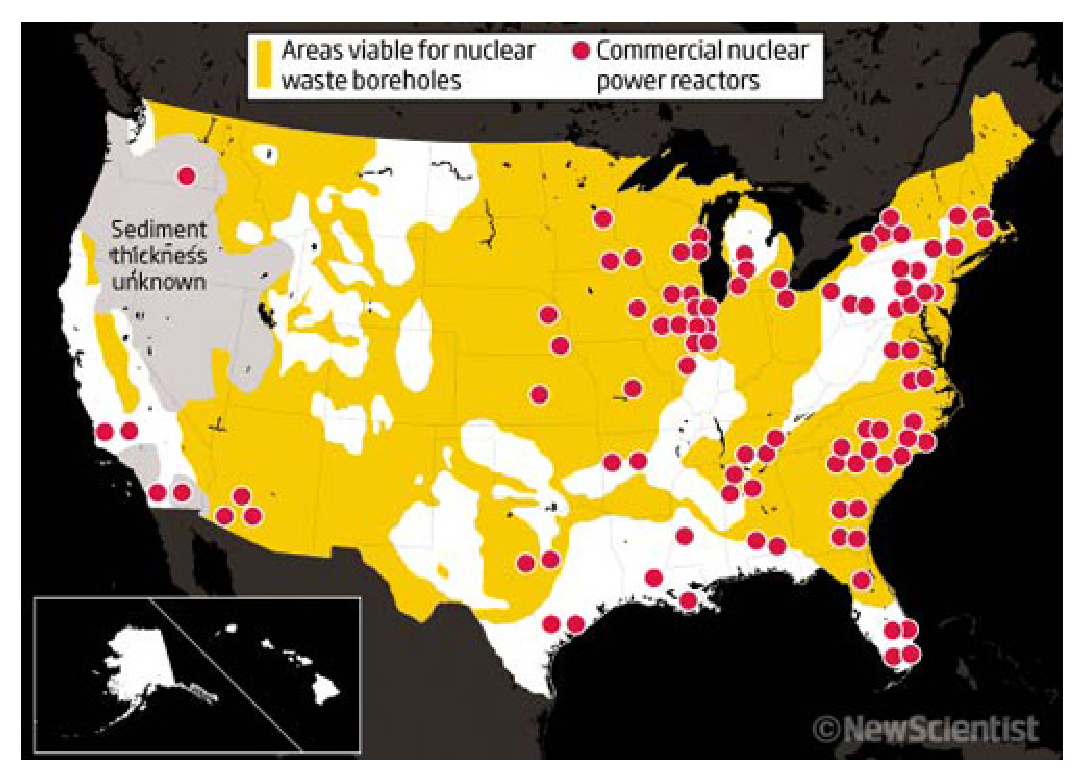
\includegraphics[width=0.8\textwidth]{boreholeNewScientist.eps}
         \caption{U.S. Crystalline Basement ref.  \cite{newscientist_where_2011}}
     \end{figure}
     \begin{figure}[h!]
         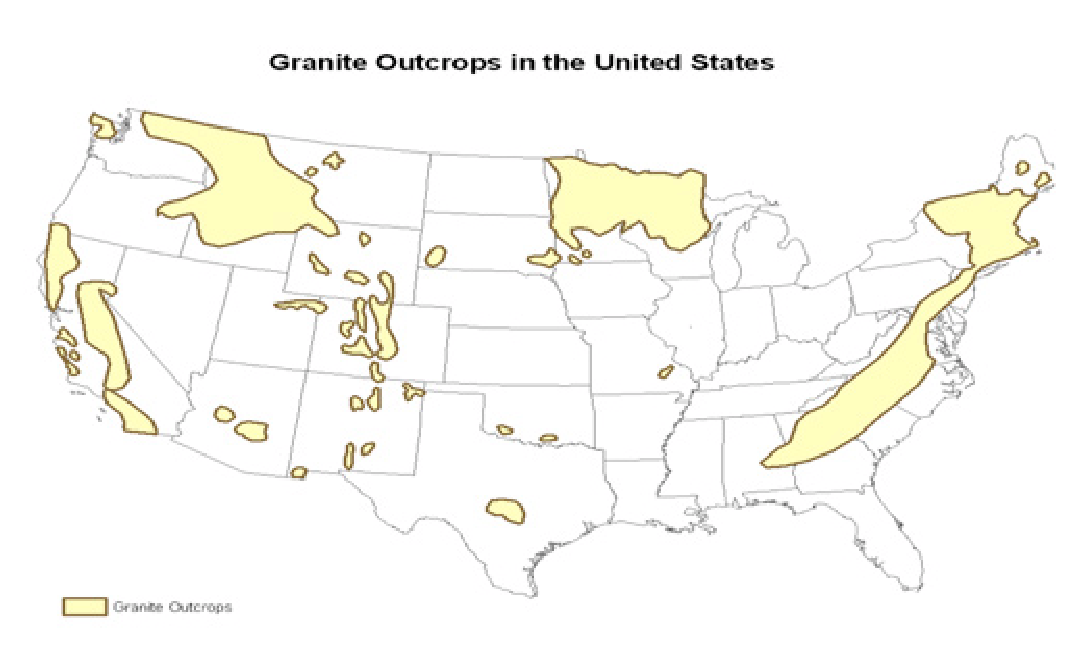
\includegraphics[width=0.8\textwidth]{graniteBush.eps}
         \caption{U.S. Granite ref. \cite{bush_economic_1976}}
     \end{figure}
   \end{minipage}
\end{frame}


\begin{frame}[ctb!]
  \frametitle{Future Fuel Cycle Options}
   % Future Fuel Cycles
    \begin{table}
      \centering
      \footnotesize{
      \begin{tabular}{|l|l|l|}
        \multicolumn{3}{c}{\textbf{Domestic Fuel Cycle Options}}\\
        \hline
        Title & Description& Challenges \\
        \hline
        Open          & Once Through         & High Temperatures, Volumes \\
                      & Current US PWR Fleet &      \\
                      & No Separations       &      \\
                      & No Recycling         &      \\
                      & Higher Burnups &      \\
        Modified Open & Partial Recycling    & Both high volumes and myriad fuel streams \\
                      & Next Gen. PWR Fleet &      \\
                      & Limited Separations  &      \\
                      & Limited Transmutation &      \\
                      & Advanced Fuel Forms  &      \\
        Closed        & Full Recycling       & Myriad fuel streams \\
                      & Full Separations &      \\
                      & Full Recycling &      \\
                      & VHTGR, SFRs, &      \\
                      & <++> &      \\
                      & <++> &      \\
                      & <++> &      \\
                      & <++> &      \\
                      & <++> &      \\
        \hline
      \end{tabular}
      \caption[Fuel Cycle Options]{Domestic Fuel Cycle Options }
      \label{tab:fco}
      }
    \end{table}
\end{frame}



\subsection{Repository Capabilities within Systems Analysis Tools}


% They just report mass flows
% or are proprietary and super long running

\begin{frame}[ctb!]
  \frametitle{Cyclus Top Level Fuel Cycle Simulator}
  % most only report mass flows.
  \begin{figure}[htbp!]
    \begin{center}
      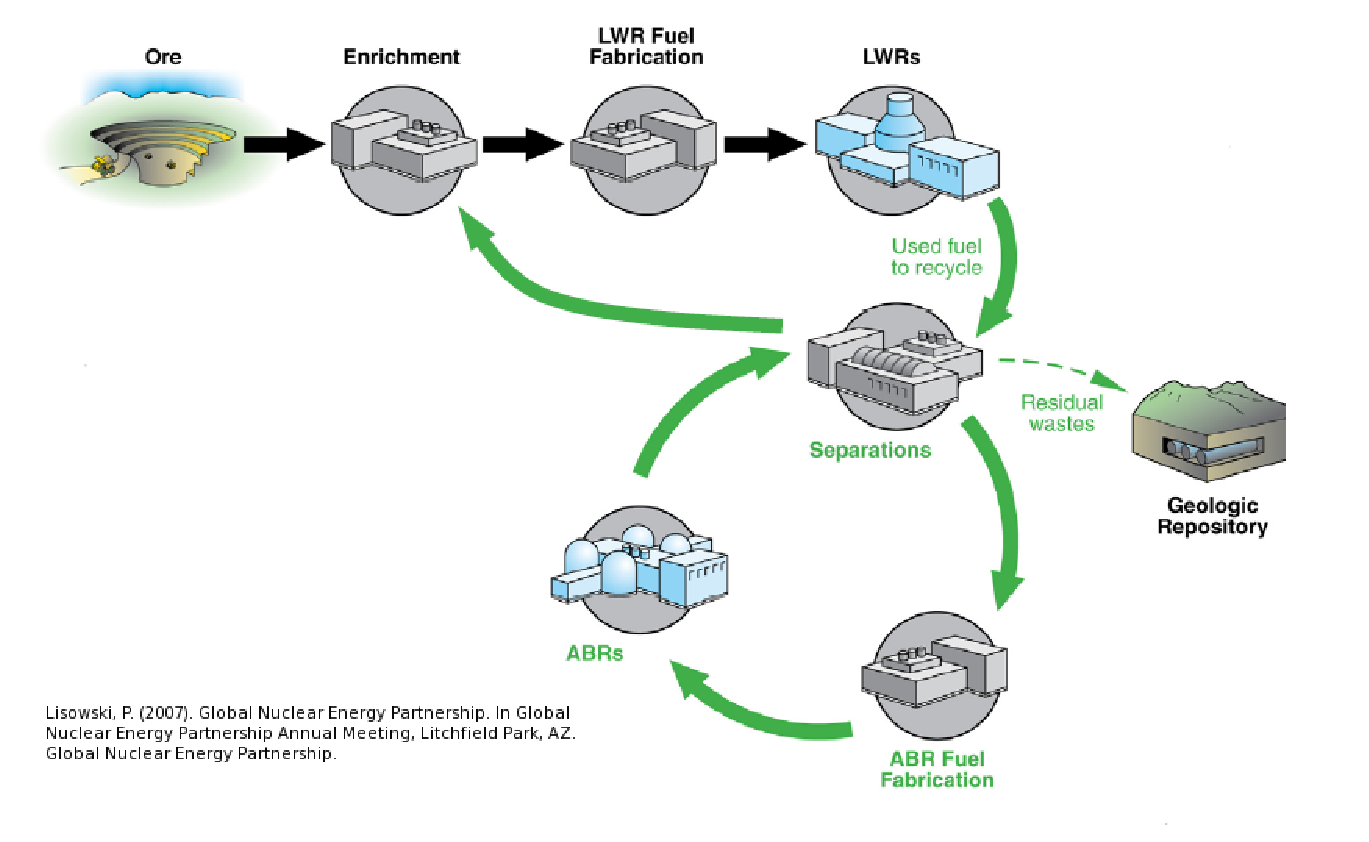
\includegraphics[height=3.5cm]{./images/simulations.eps}
    \end{center}
    \caption{Top level simulators are intended to model the collective 
    behavior of various fuel cycle decisions and 
    strategies \cite{lisowski_global_2007}.}
    \label{fig:simulation}
  \end{figure}
  \begin{figure}[htbp!]
    \begin{center}
      
\includegraphics[height=1cm]{./images/cycluslogo.eps}
    \end{center}
    \caption{ cyclus.github.com \cite{huff_cyclus_2013}.}
    \label{fig:simulation}
  \end{figure}
\end{frame}

\begin{frame}[ctb!]
  \frametitle{Need For an Integrated Repository Model}

  %        File: systools_tab.tex
%     Created: Mon Aug 29 09:00 AM 2011 C
% Last Change: Mon Aug 29 09:00 AM 2011 C
%
\begin{table}
  \centering
  \footnotesize{
  \begin{tabular}{|l|l|c|c|c|}
    \multicolumn{5}{c}{\textbf{Repository Capabilities within Systems Analysis Tools}}\\
    \hline
    Tool & Institution & Fuel Disposition & Radionuclide Transport & Heat Transport  \\
    \hline
    NUWASTE\cite{abkowitz_nuclear_2010} & NWTRB & yes & no & no \\
    VISION \cite{yacout_vision_2006} & INL   & yes & no & YMR only \\
    DANESS \cite{van_den_durpel_daness:_2006} & ANL   & no & no & no \\
    COSI   \cite{boucher_international_2010} & CEA   & yes & no & yes \\
    NFCSim \cite{schneider_nfcsim_2004} & LANL  & no & no & no \\
    CAFCA  \cite{guerin_benchmark_2009} & MIT   & no & no & no \\
    ORION  \cite{guerin_benchmark_2009} & BNL   & no & no & no \\
    TSM    \cite{turner_discrete_2010} & OCRWM & yes & no & YMR only \\
    \hline
  \end{tabular}
  \caption[System Tools]{System tools are lacking in radionuclide transport and  
  heat transport calculations in generic geologic media.}
  \label{tab:systools}
  }
\end{table}




\end{frame}


\begin{frame}[ctb!]
\frametitle{Contributions from This Work}

This work has provided a platform capable of bridging the gap between fuel cycle 
simulation and repository performance analysis.

  \begin{itemize}
  \item Conducted thermal transport sensitivity analyses. \cite{huff_numerical_2012, huff_benchmarking_2012}
  \item Conducted contaminant transport sensitivity analyses. \cite{huff_key_2012}
  \item \Cyder acheived integration with a fuel cycle simulator.
  \item Abstracted physical models of thermal and contaminant transport. \cite{huff_hydrologic_2013}
  \item Demonstrated dominant physics of those models in \Cyder, integrated 
  with \Cyclus. \cite{huff_dynamic_2013, huff_cyclus_2013}
  \item Published source code, documentation, and testing to facilitate 
  extension by external developers. \cite{huff_cyder_2013}
  \end{itemize}
\end{frame}


\subsection{Conceptual Discussion of Disposal Environments}
% layouts
% EBS choices
% Geologies


\begin{frame}[ctb!]
  \frametitle{Clay Disposal Environments}

  \begin{figure}[h!]
    \begin{center}
      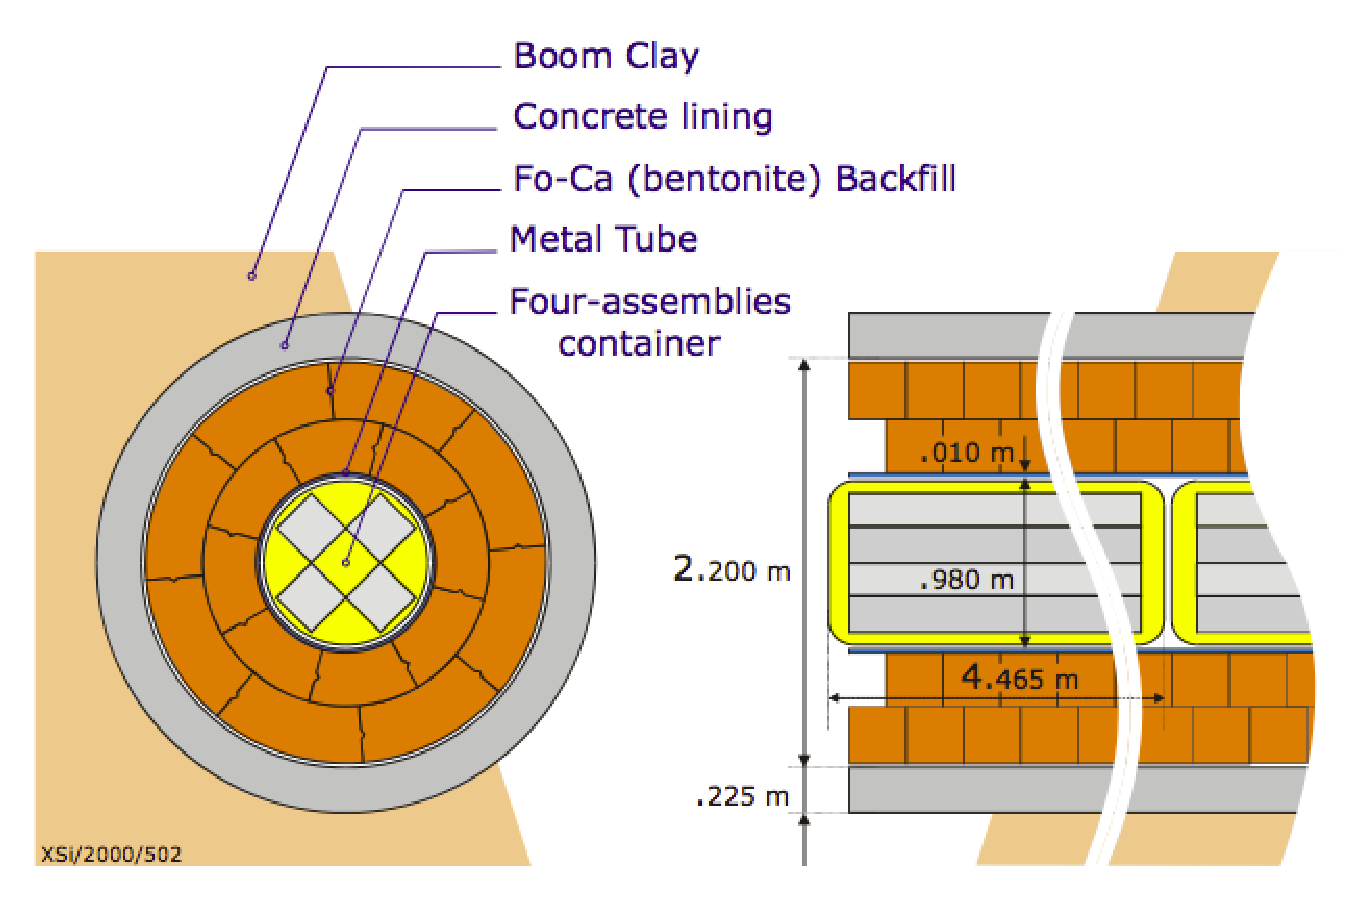
\includegraphics[height=.7\textheight]{belgianClayRedImp.eps}
    \end{center}
    \caption{Belgian reference concept in Boom Clay 
    \cite{von_lensa_red-impact_2005}.}
    \label{fig:belgianClayRedImp}
  \end{figure}

\end{frame}

\begin{frame}[ctb!]
  \frametitle{Granite Disposal Environments}

  \begin{figure}[h!]
    \begin{center}
      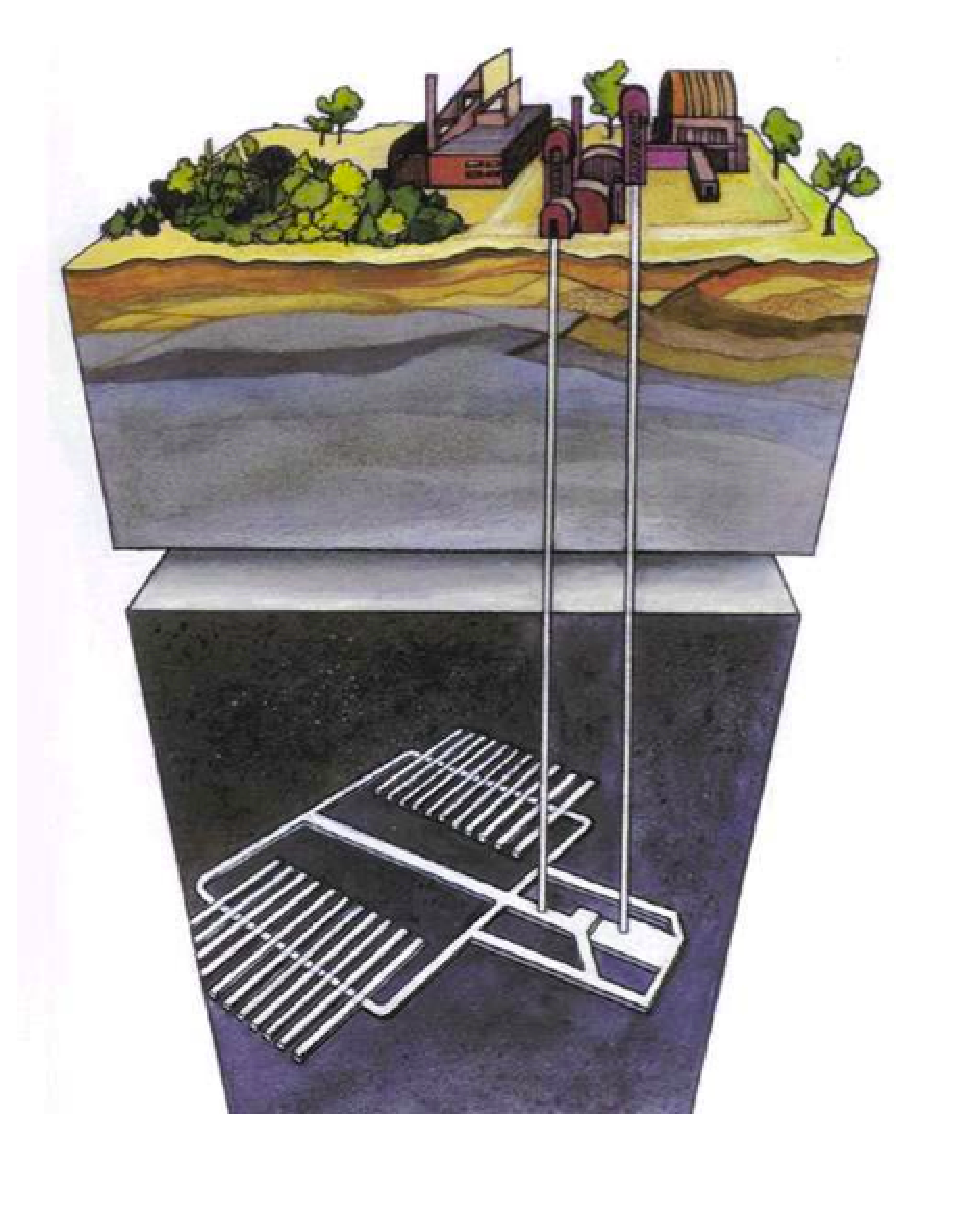
\includegraphics[height=.7\textheight]{czechGraniteRedImp.eps}
    \end{center}
    \caption{Czech reference concept in Granite 
    \cite{von_lensa_red-impact_2005}.}
    \label{fig:czechGraniteRedImp}
  \end{figure}

\end{frame}

\begin{frame}[ctb!]
  \frametitle{Salt Disposal Environments}

  \begin{figure}[h!]
    \begin{center}
      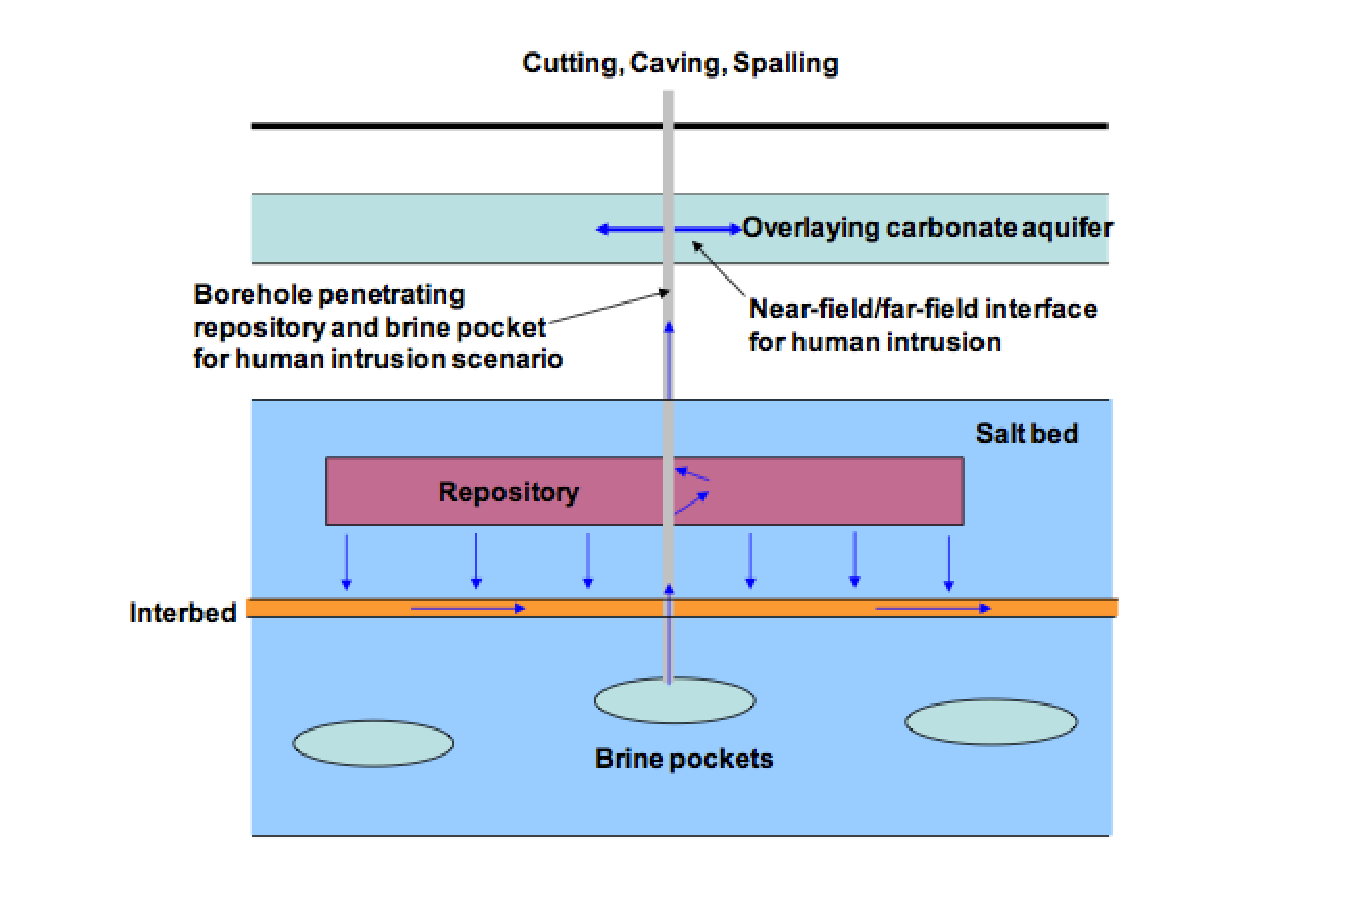
\includegraphics[height=.7\textheight]{saltGPAM.eps}
    \end{center}
    \caption{DOE-NE Used Fuel Disposition Campaign  concept in 
    Salt \cite{clayton_generic_2010}.}
    \label{fig:saltGPAM}
  \end{figure}

\end{frame}

\begin{frame}[ctb!]
  \frametitle{Deep Borehole Disposal Environment}

  \begin{figure}[h!]
    \begin{center}
      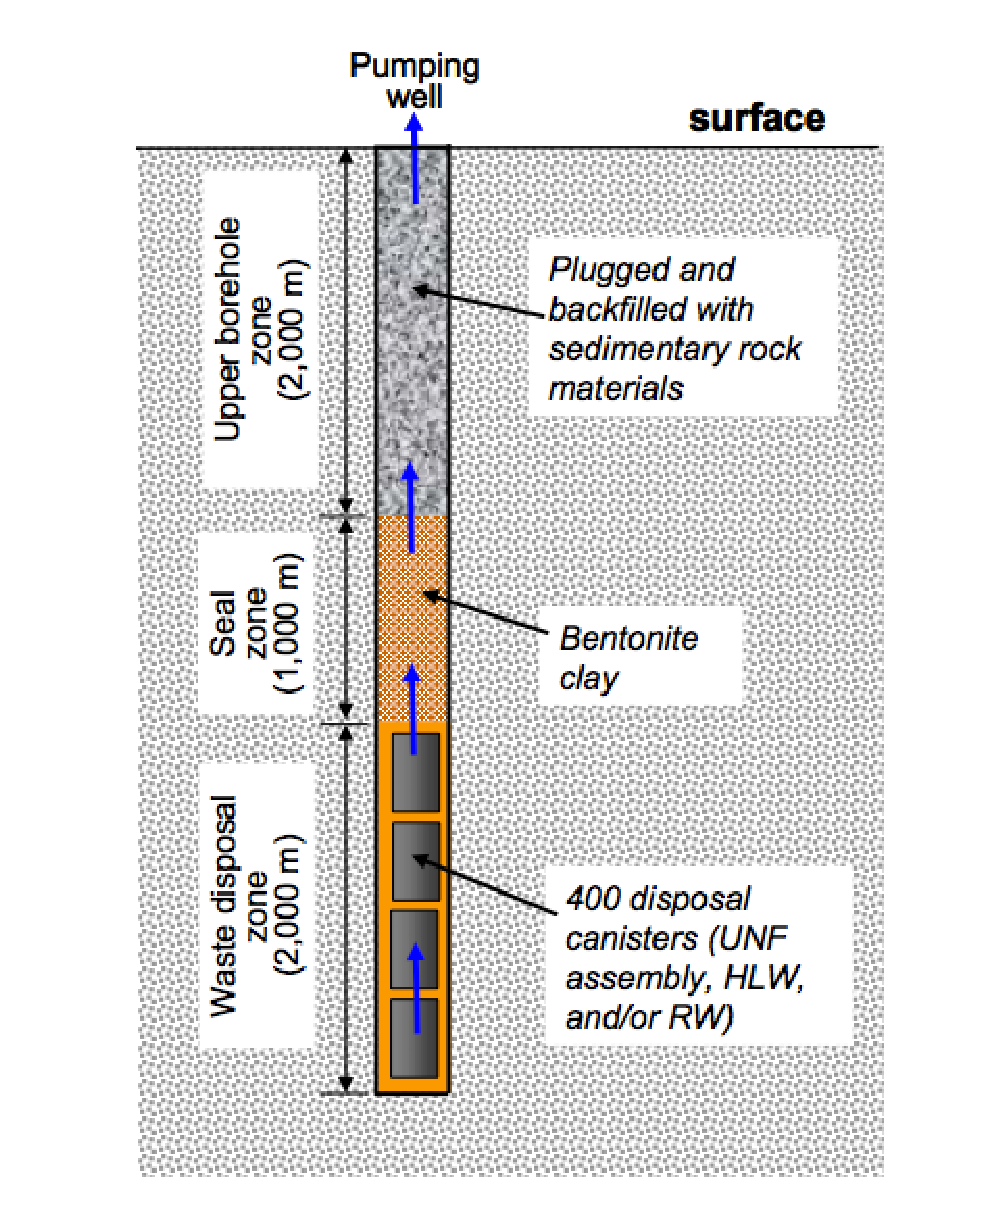
\includegraphics[height=.7\textheight]{boreholeGPAM.eps}
    \end{center}
    \caption{DOE-NE Used Fuel Disposition Campaign Deep Borehole concept 
    \cite{clayton_generic_2010}.}
    \label{fig:boreholeGPAM}
  \end{figure}

\end{frame}


\begin{frame}
  \frametitle{Repository Layouts}

  \begin{minipage}{0.49\textwidth}
    \begin{figure}[h!]
      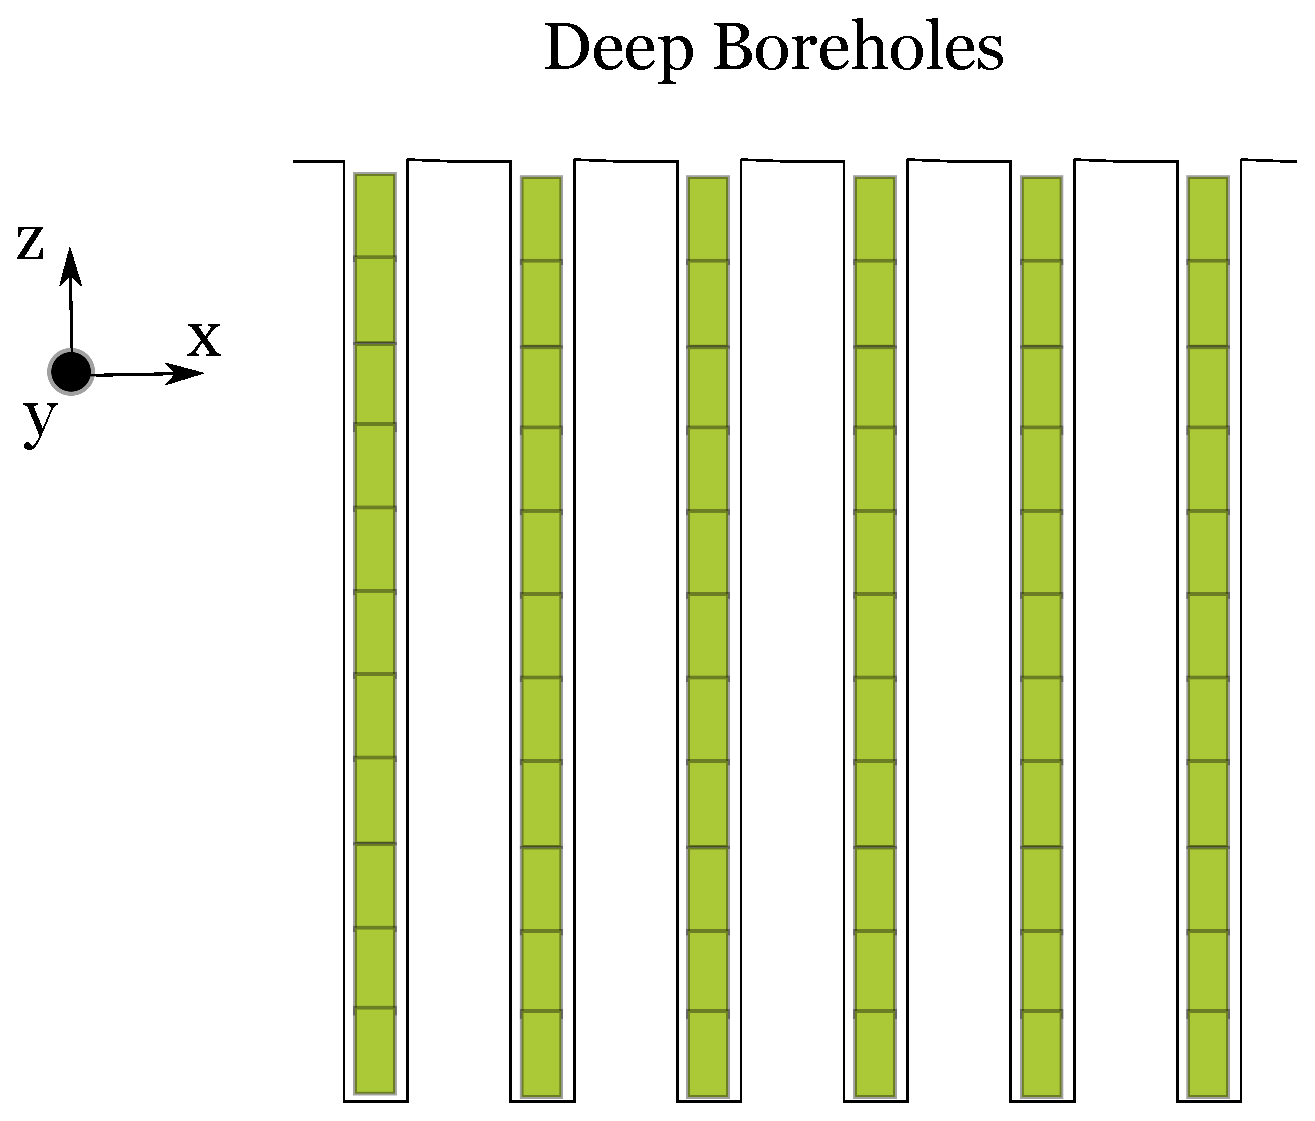
\includegraphics[width=0.75\textwidth]{boreholes.eps}
    \end{figure}
    \begin{figure}[h!]
      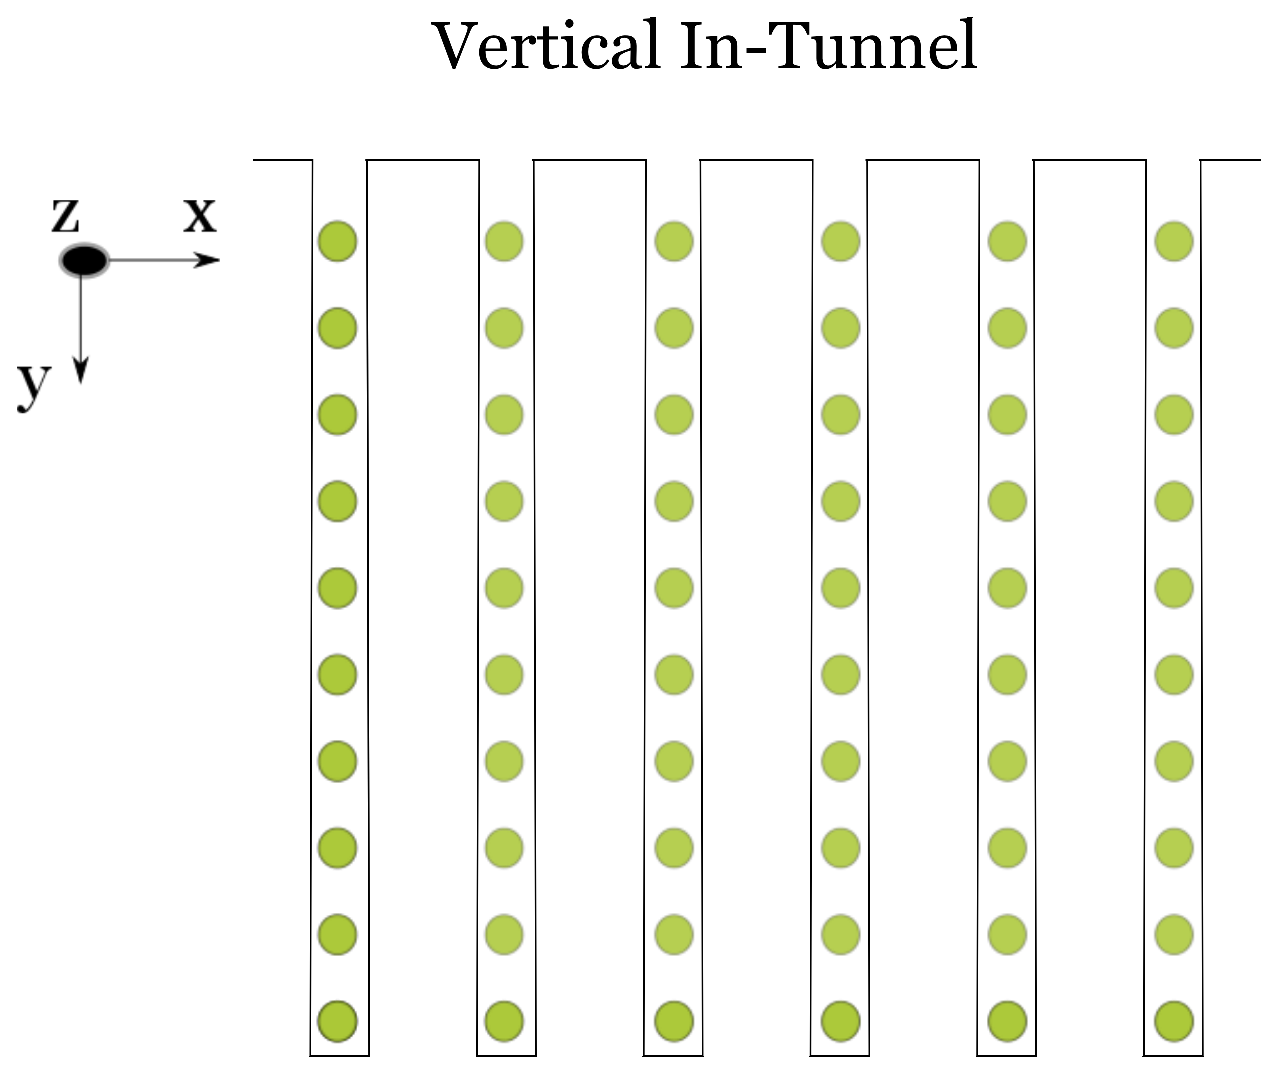
\includegraphics[width=0.75\textwidth]{vertical.eps}
    \end{figure}
  \end{minipage}
  \hspace{0.01cm}
  \begin{minipage}{0.49\textwidth}
    \begin{figure}[h!]
      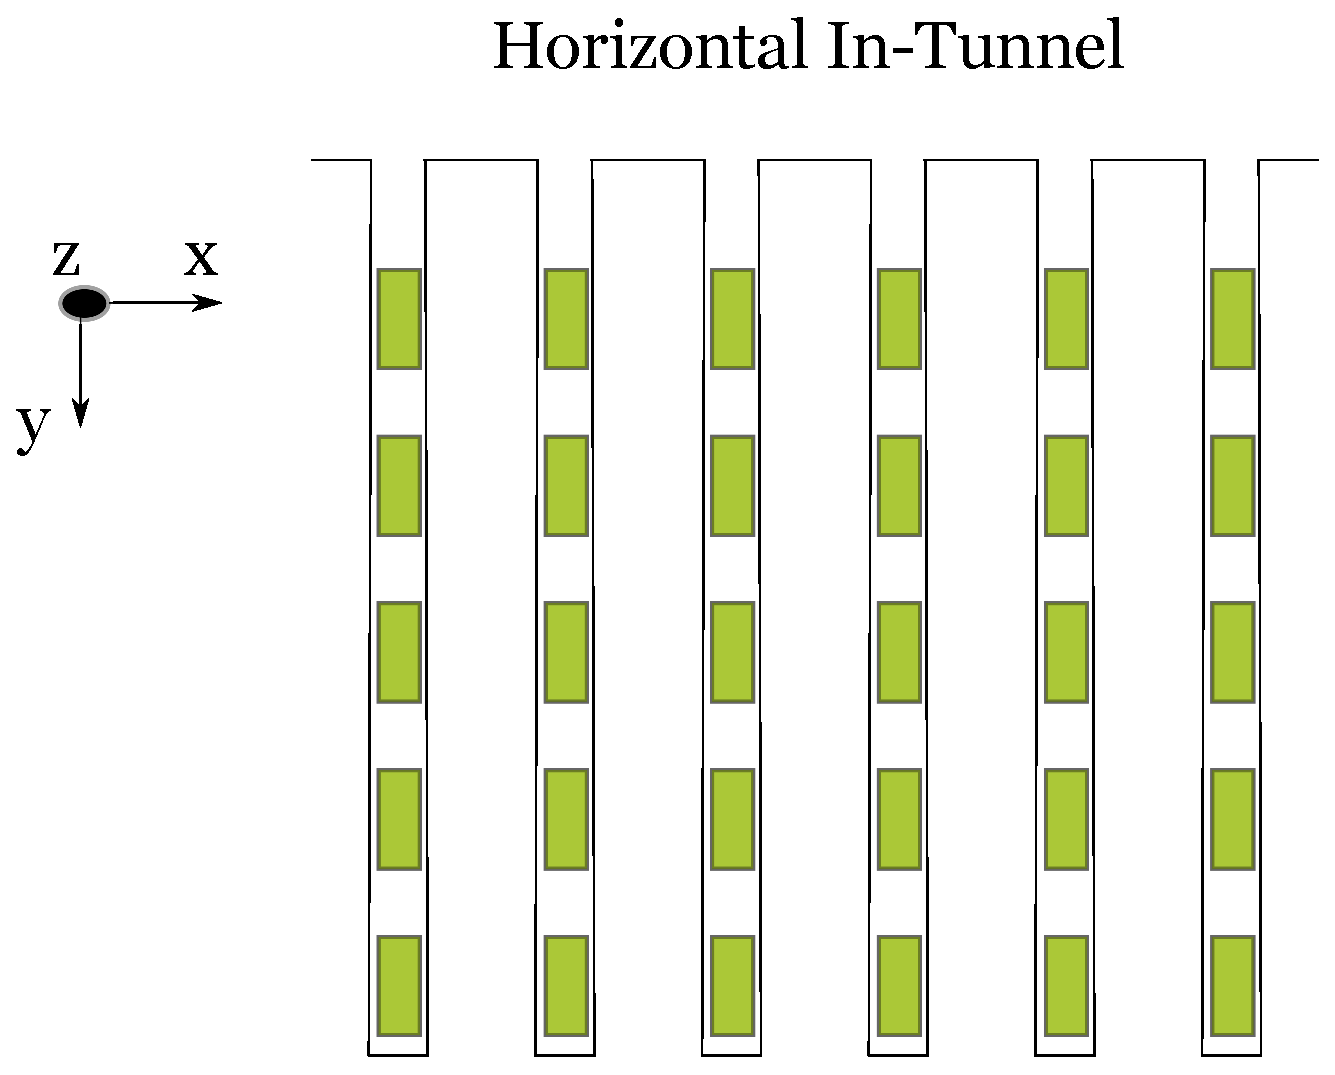
\includegraphics[width=0.8\textwidth]{horizontal.eps}
    \end{figure}
    \begin{figure}[h!]
      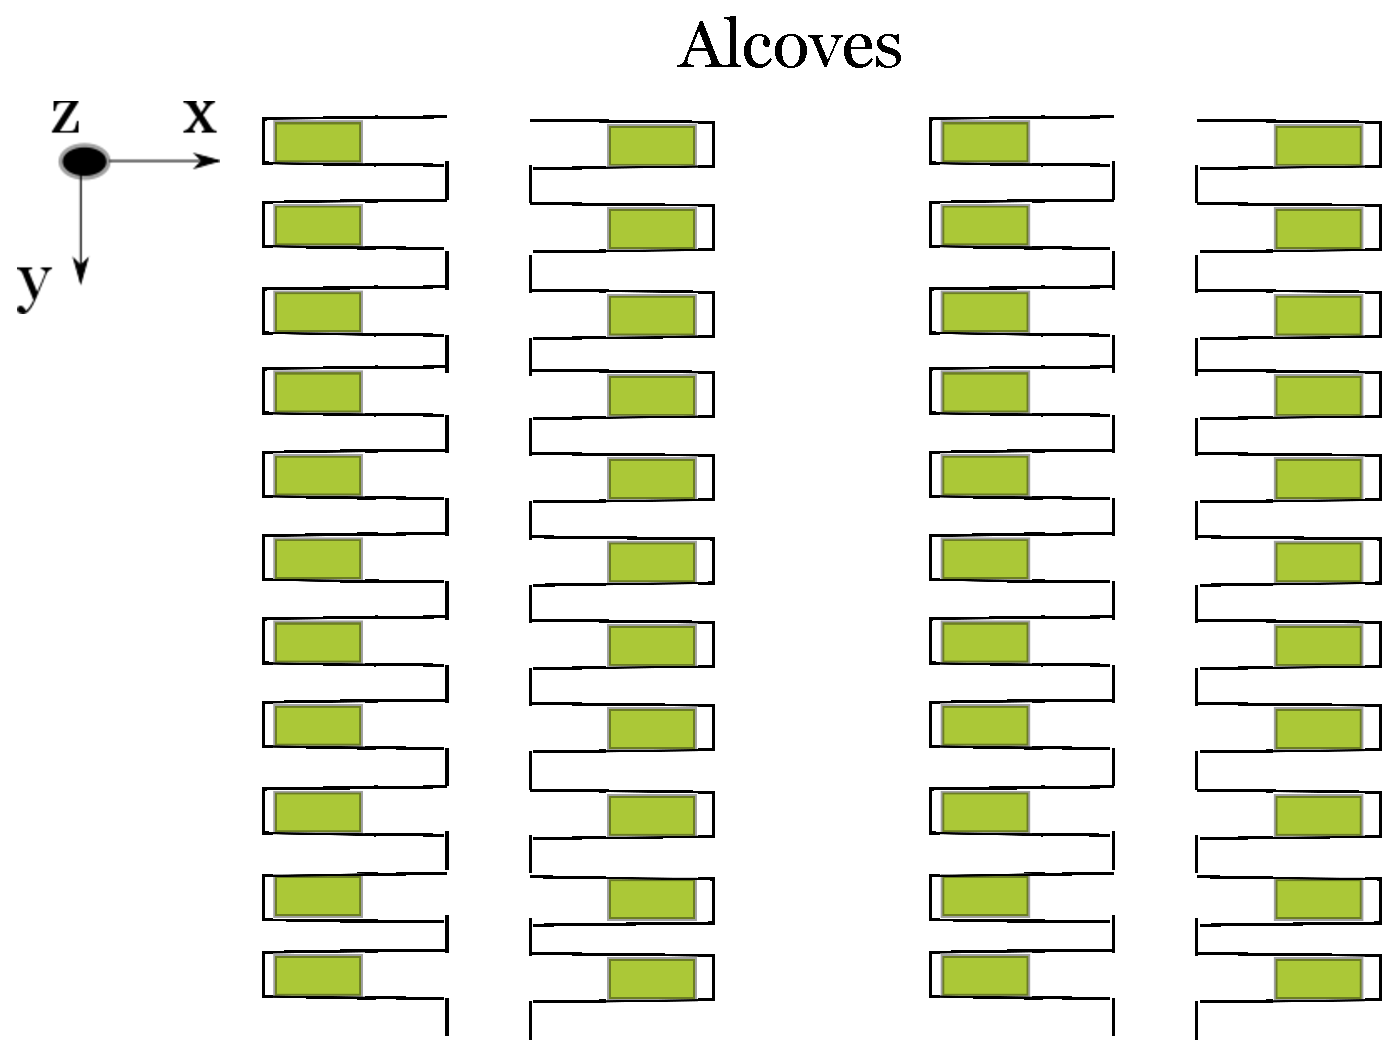
\includegraphics[width=0.8\textwidth]{alcoves.eps}
    \end{figure}
  \end{minipage}

\end{frame}

\begin{frame}[ctb!]
  \frametitle{All Disposal Environments}
  % Table
  %        File: geos_tab.tex
%     Created: Thu Aug 04 11:00 AM 2011 C
% Last Change: Thu Aug 04 11:00 AM 2011 C
%
\begin{table}[h!]
  \centering
  \footnotesize{
  \begin{tabular}{|l|r|r|r|r|}
    \multicolumn{5}{c}{\textbf{Features of Various Concepts}}\\
    \hline
    Feature & Clay & Granite & Salt & Deep Borehole \\ 
    \hline
    \multicolumn{5}{|c|}{\textbf{Hydrology}}\\
    \hline
    Total Porosity $[\%]$    & 34-60  & 0.1 & 0.5 & 0-0.5 \\ 
    Eff. Porosity $[\%]$ & 0.5-5 & 0.0005 & 0.1 & 0.00005-0.01 \\ 
    Conductivity$[m/s]$ & $10^{-11} - 10^{-9}$ & 
    $10^{-6}-10^{-5}$ & $10^{-12}-10^{-10}$ & 
    $10^{-13}-10^{-4}$ \\ 
    Fracturation & none & high & none & low at depth \\ 
    \hline
    \hline
    \multicolumn{5}{|c|}{\textbf{Geochemistry}}\\
    \hline
    Reducing & Near \& Far Field & NF only  & NF only & NF only \\
    Oxidizing & none & Slight in FF & Slight in FF & Slight in FF \\
    Salinity & higher at depth & higher at depth & high & high \\
    pH & $\sim7$ & $\ge7$ & $\ge7$ & $\sim7$ \\
    \hline
    \hline
    \multicolumn{5}{|c|}{\textbf{Design}}\\
    \hline
    Waste Package & Steel, Cu & Steel, Cu & Steel & Steel,Cement \\
    Buffer & -,Fo-Ca,Cement & Fo-Ca,Cement & Crushed Salt & -,Fo-Ca,Cement\\ 
    Depth & 100-500 m & 100-500 m & 100-500m & 3-5km \\ 
    Emplacement & Vert.,Horiz,Alcove & Vert.,Horiz. & Alcove & Vert. \\ 
    Packages/Gallery & one, many & one, many & one, two & 400 \\ 
    \hline
    \hline
    \multicolumn{5}{|c|}{\textbf{Thermal Behavior}}\\
    \hline
    Buffer Limit $[^{\circ}C]$ & 100 (Fo-Ca) & 100 (Fo-Ca) & 180 & 100 (Fo-Ca) \\ 
    Host Limit $[^{\circ}C]$   & 100 (alteration)  & 200 (cracking) & 180 (brines) & none \\ 
    Conductivity $[\frac{W}{m{\cdot}K}]$ & $1-2$ & $2-4$ & $\sim4$  & $2-4$ \\ 
    Coalesence & yes & no & yes & no \\ 
    \hline
  \end{tabular}
  }
  \label{tab:geos_tab}
\end{table}
%  \cite{stober_hydraulic_2006} 

\end{frame}


\section{Current Work}
\subsection{Demonstration Case}


\begin{frame}[ctb!]
  \frametitle{Demonstration Case : Code Development}
  Empty Concept

  Interfaces, information passing, module loading. Not in that order.

  Information passing tests, Database writing tests, module loading tests.
\end{frame}

\subsection{Base Case}


\begin{frame}
  \frametitle{Base Case : Nested Components}
  \begin{itemize}
    \item Waste Form
      \begin{itemize}
        \item Mixed Cell with  Rate Based Degradation Model
        \item Glass and UOx Data
      \end{itemize}
    \item Waste Package
      \begin{itemize}
        \item Rate Based Failure Model
        \item Steel and Copper Data
      \end{itemize}
    \item Buffer
      \begin{itemize}
        \item Mixed Cell with  Rate Based Degradation Model
        \item Bentonite (Fo-Ca), Salt, and Cement Data
      \end{itemize}
    \item Geology
      \begin{itemize}
        \item Ogata and Banks 1D Permeable Porous Medium Solute Transport
        \item Data for Clay, Granite, Salt, and Crystalline Basement
      \end{itemize}
  \end{itemize}
\end{frame}

\begin{frame}[ctb!]
  \frametitle{Base Case : Components}
  \begin{figure}[h!]
      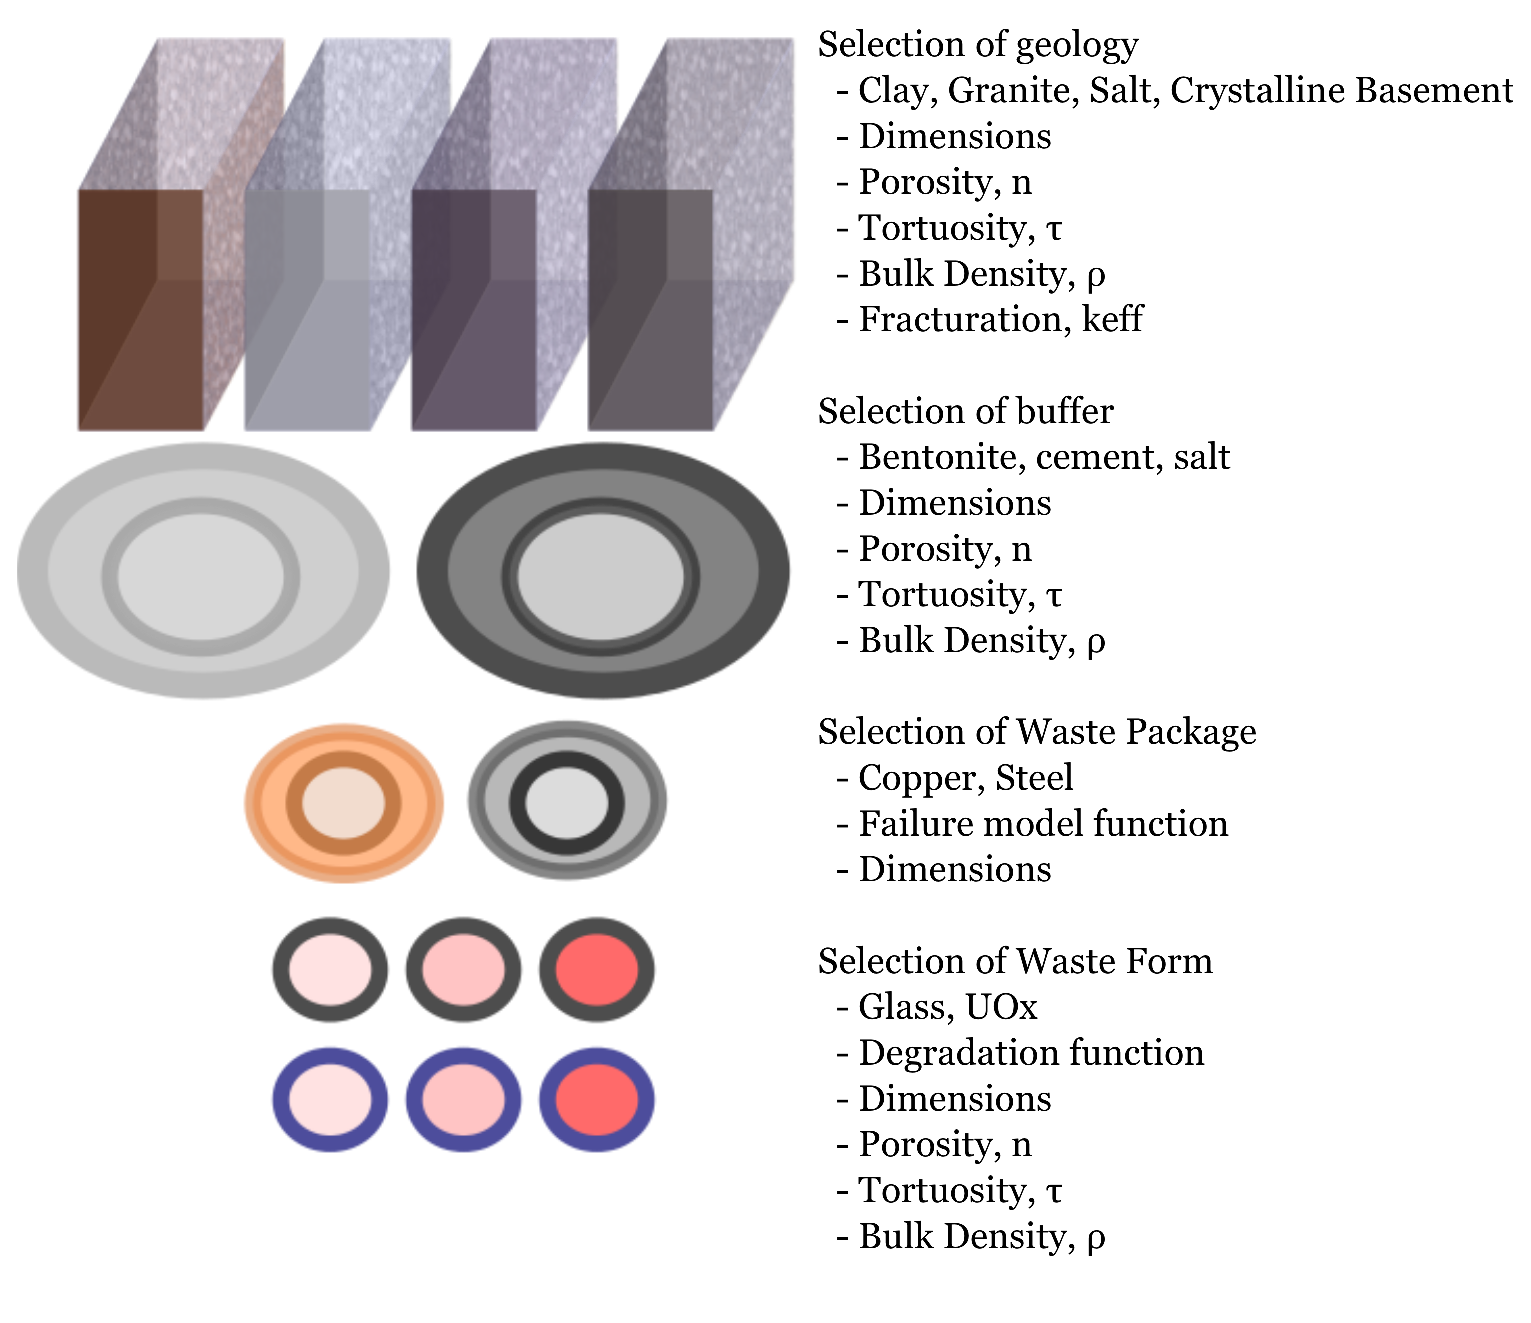
\includegraphics[height=0.8\textheight]{./images/components.eps}
  \end{figure}
\end{frame}

\begin{frame}[ctb!]
  \frametitle{Base Case : Waste Form Abstraction}
  \begin{minipage}{0.45\textwidth}
    \begin{figure}[h!]
      \begin{center}
        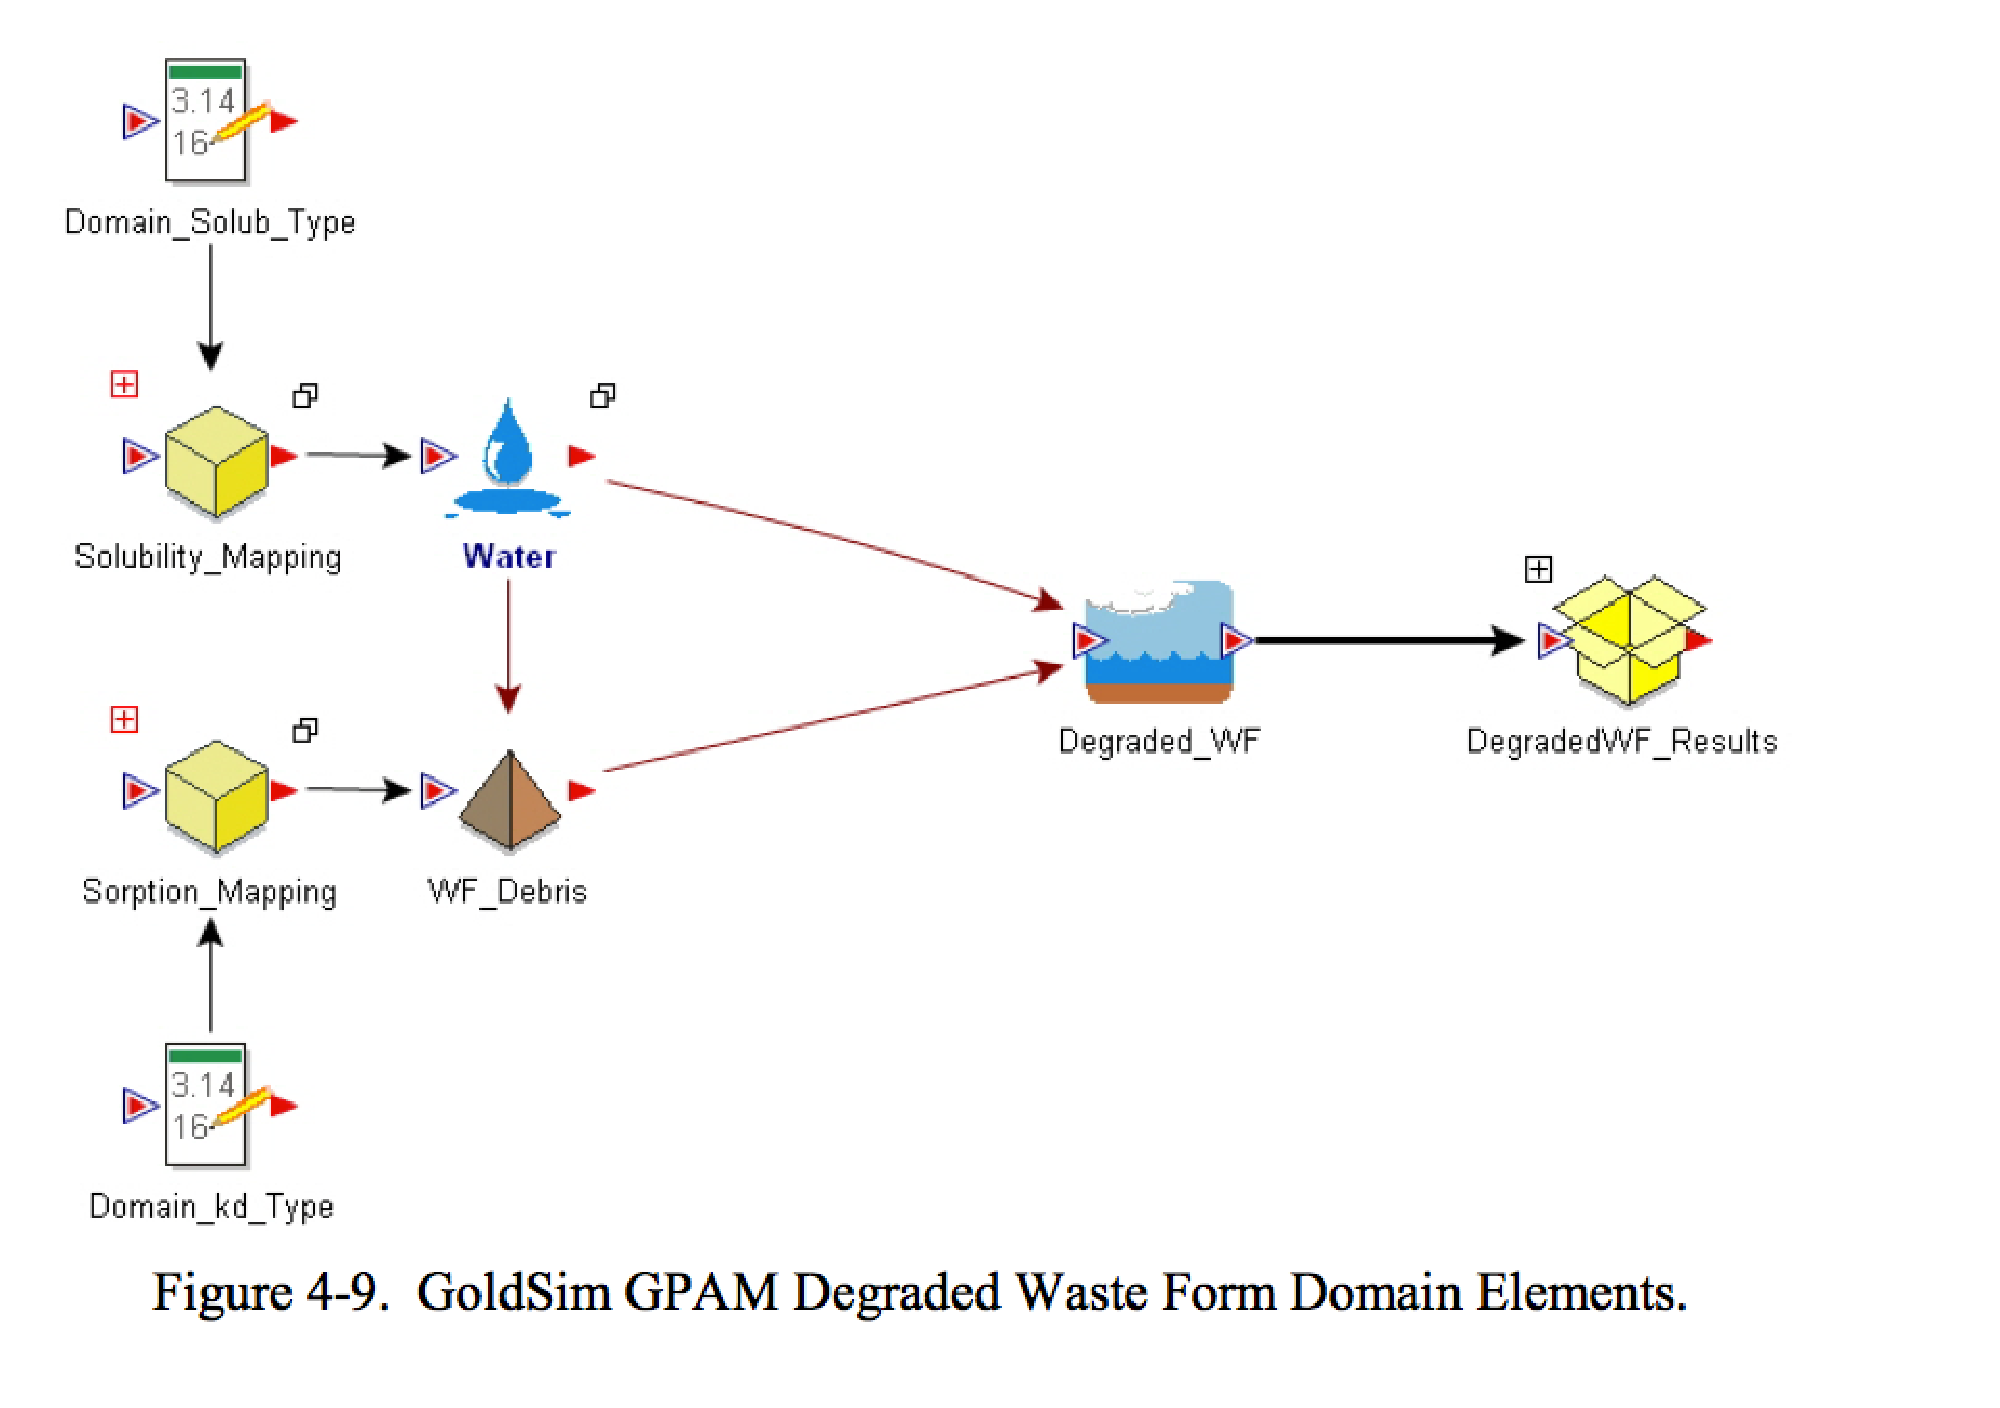
\includegraphics[width=\textwidth]{./images/wf.eps}
      \end{center}
    \end{figure}
  \end{minipage}
  \hspace{0.01cm}\large{$\rightarrow$}\hspace{0.01cm}
  \begin{minipage}{0.45\textwidth}
    \begin{figure}[h!]
      \begin{center}
        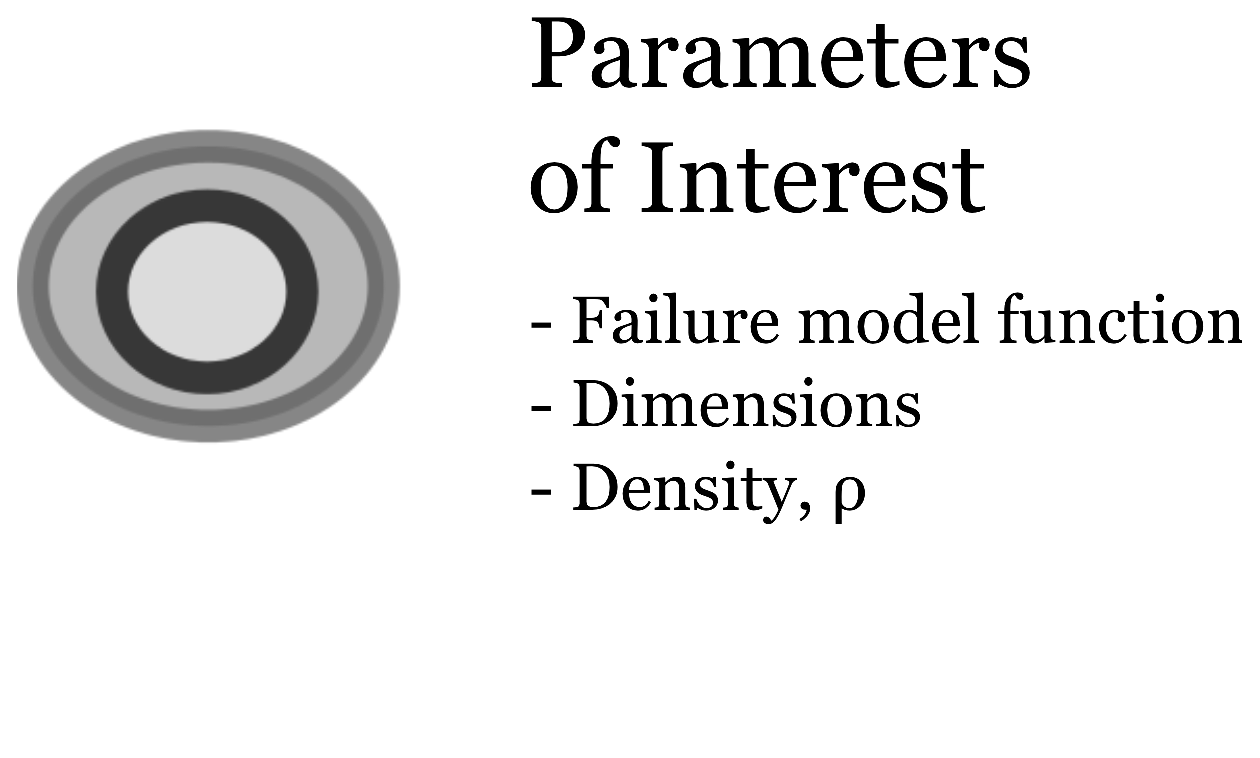
\includegraphics[width=\textwidth]{./images/abstractionWF.eps}
      \end{center}
    \end{figure}
  \end{minipage}
\end{frame}

\begin{frame}[ctb!]
  \frametitle{Base Case : Waste Package Abstraction}
  \begin{minipage}{0.45\textwidth}
    \begin{figure}[h!]
      \begin{center}
        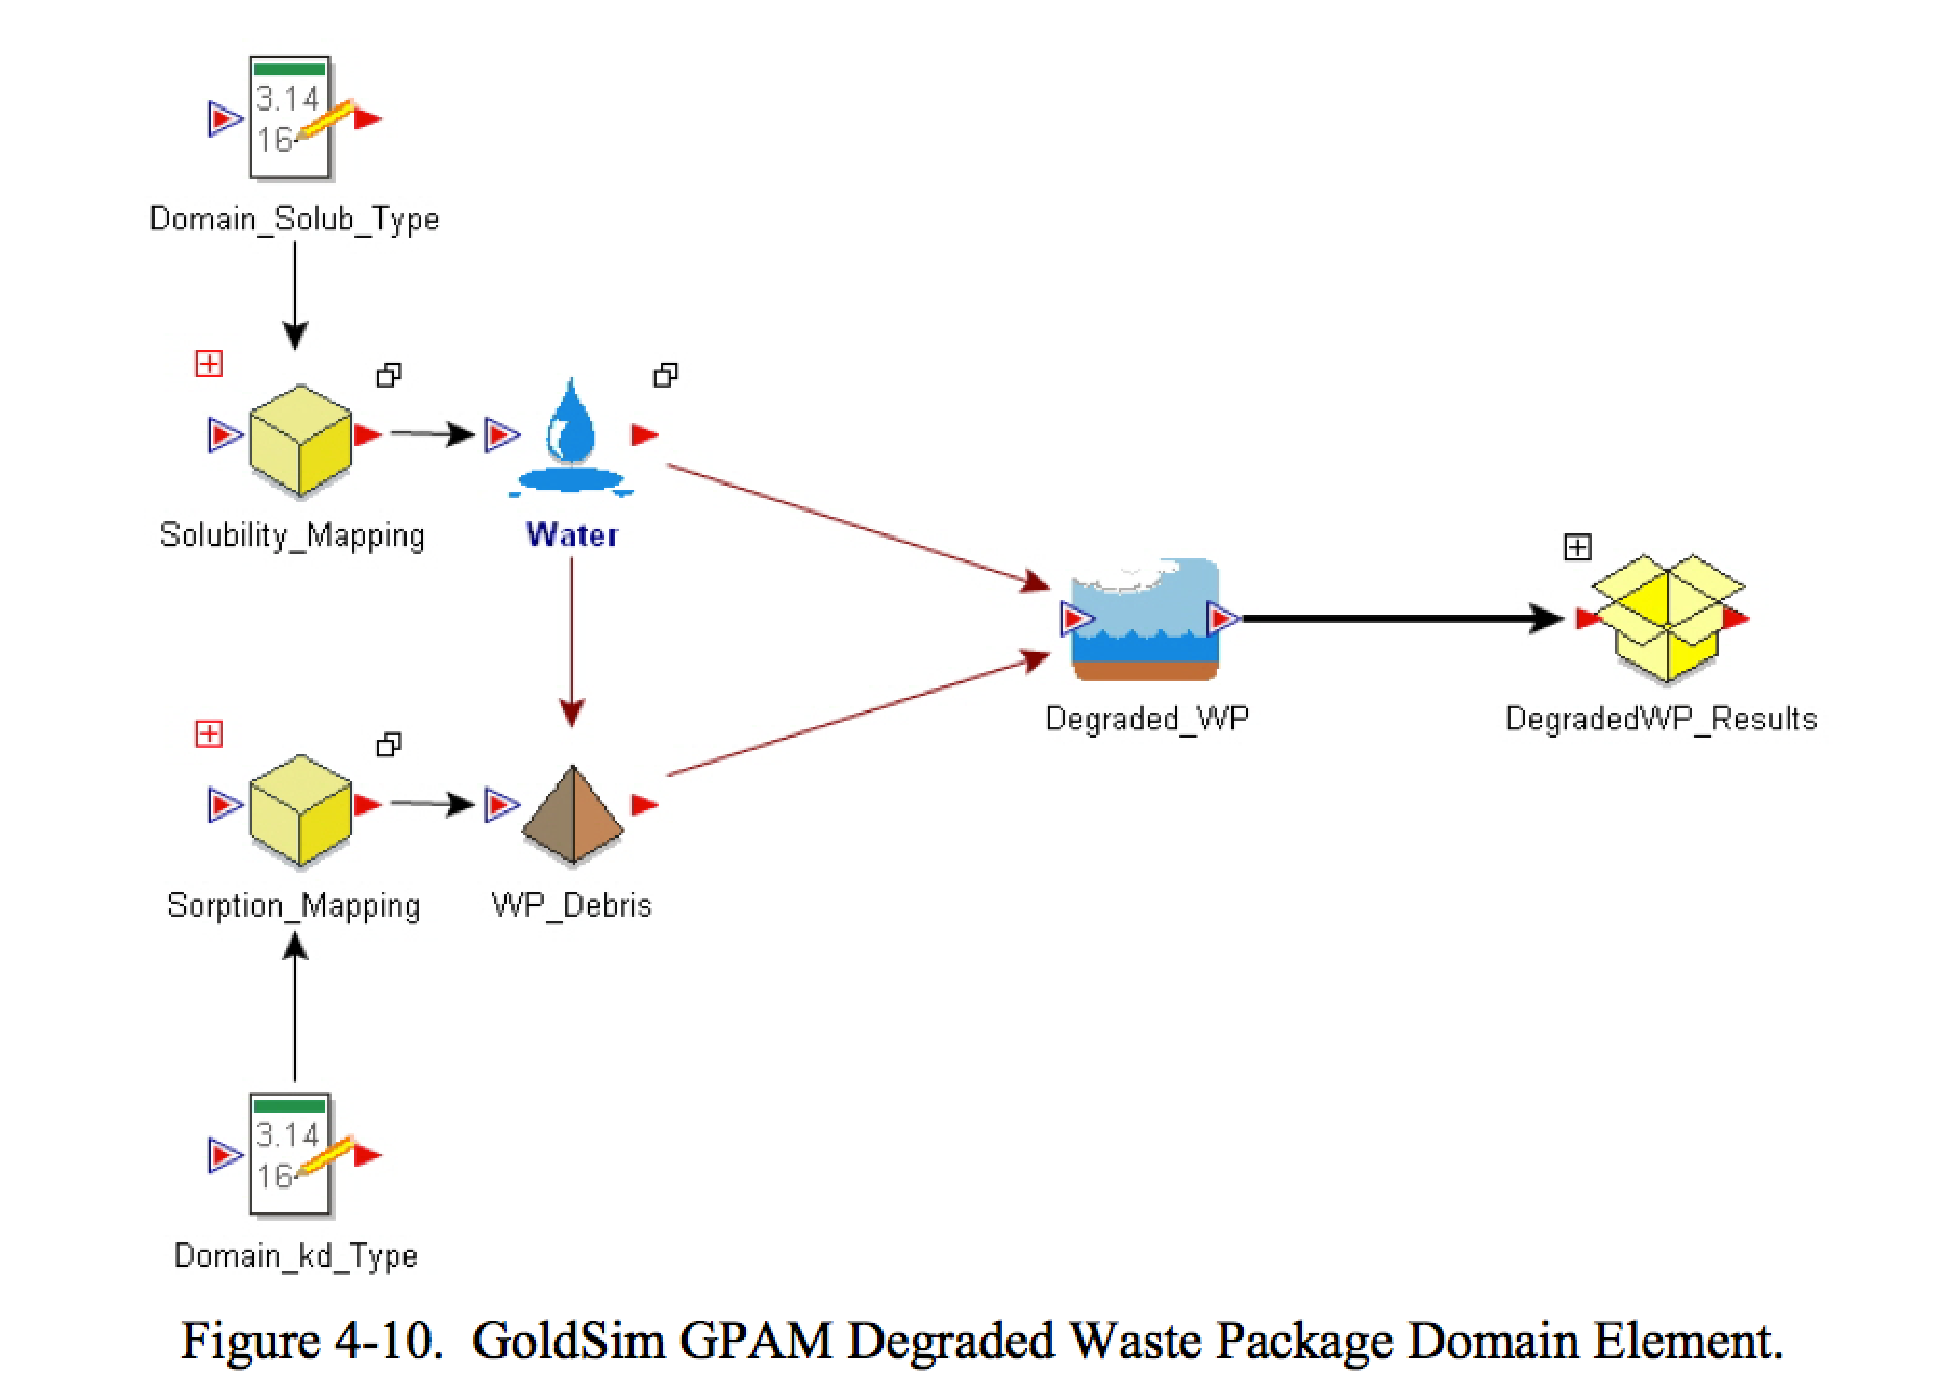
\includegraphics[width=\textwidth]{./images/wp.eps}
      \end{center}
    \end{figure}
  \end{minipage}
  \hspace{0.01cm}\large{$\rightarrow$}\hspace{0.01cm}
  \begin{minipage}{0.45\textwidth}
    \begin{figure}[h!]
      \begin{center}
        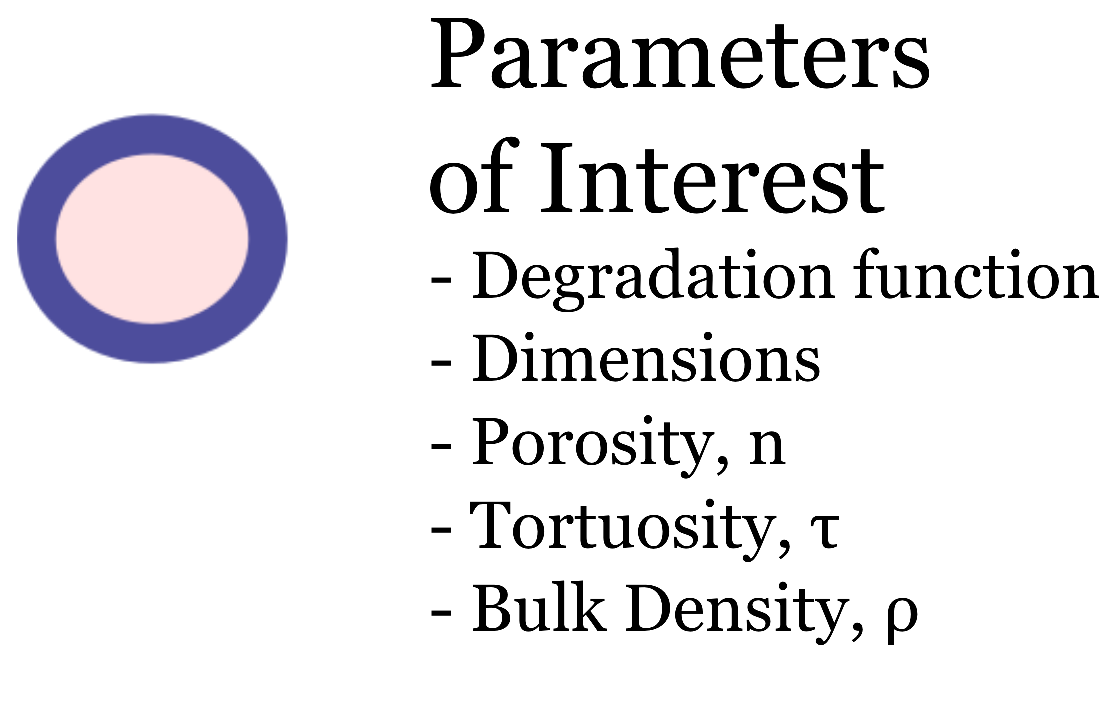
\includegraphics[width=\textwidth]{./images/abstractionWP.eps}
      \end{center}
    \end{figure}
  \end{minipage}
\end{frame}

\begin{frame}[ctb!]
  \frametitle{Base Case : Buffer Abstraction}
  \begin{minipage}{0.45\textwidth}
    \begin{figure}[h!]
      \begin{center}
        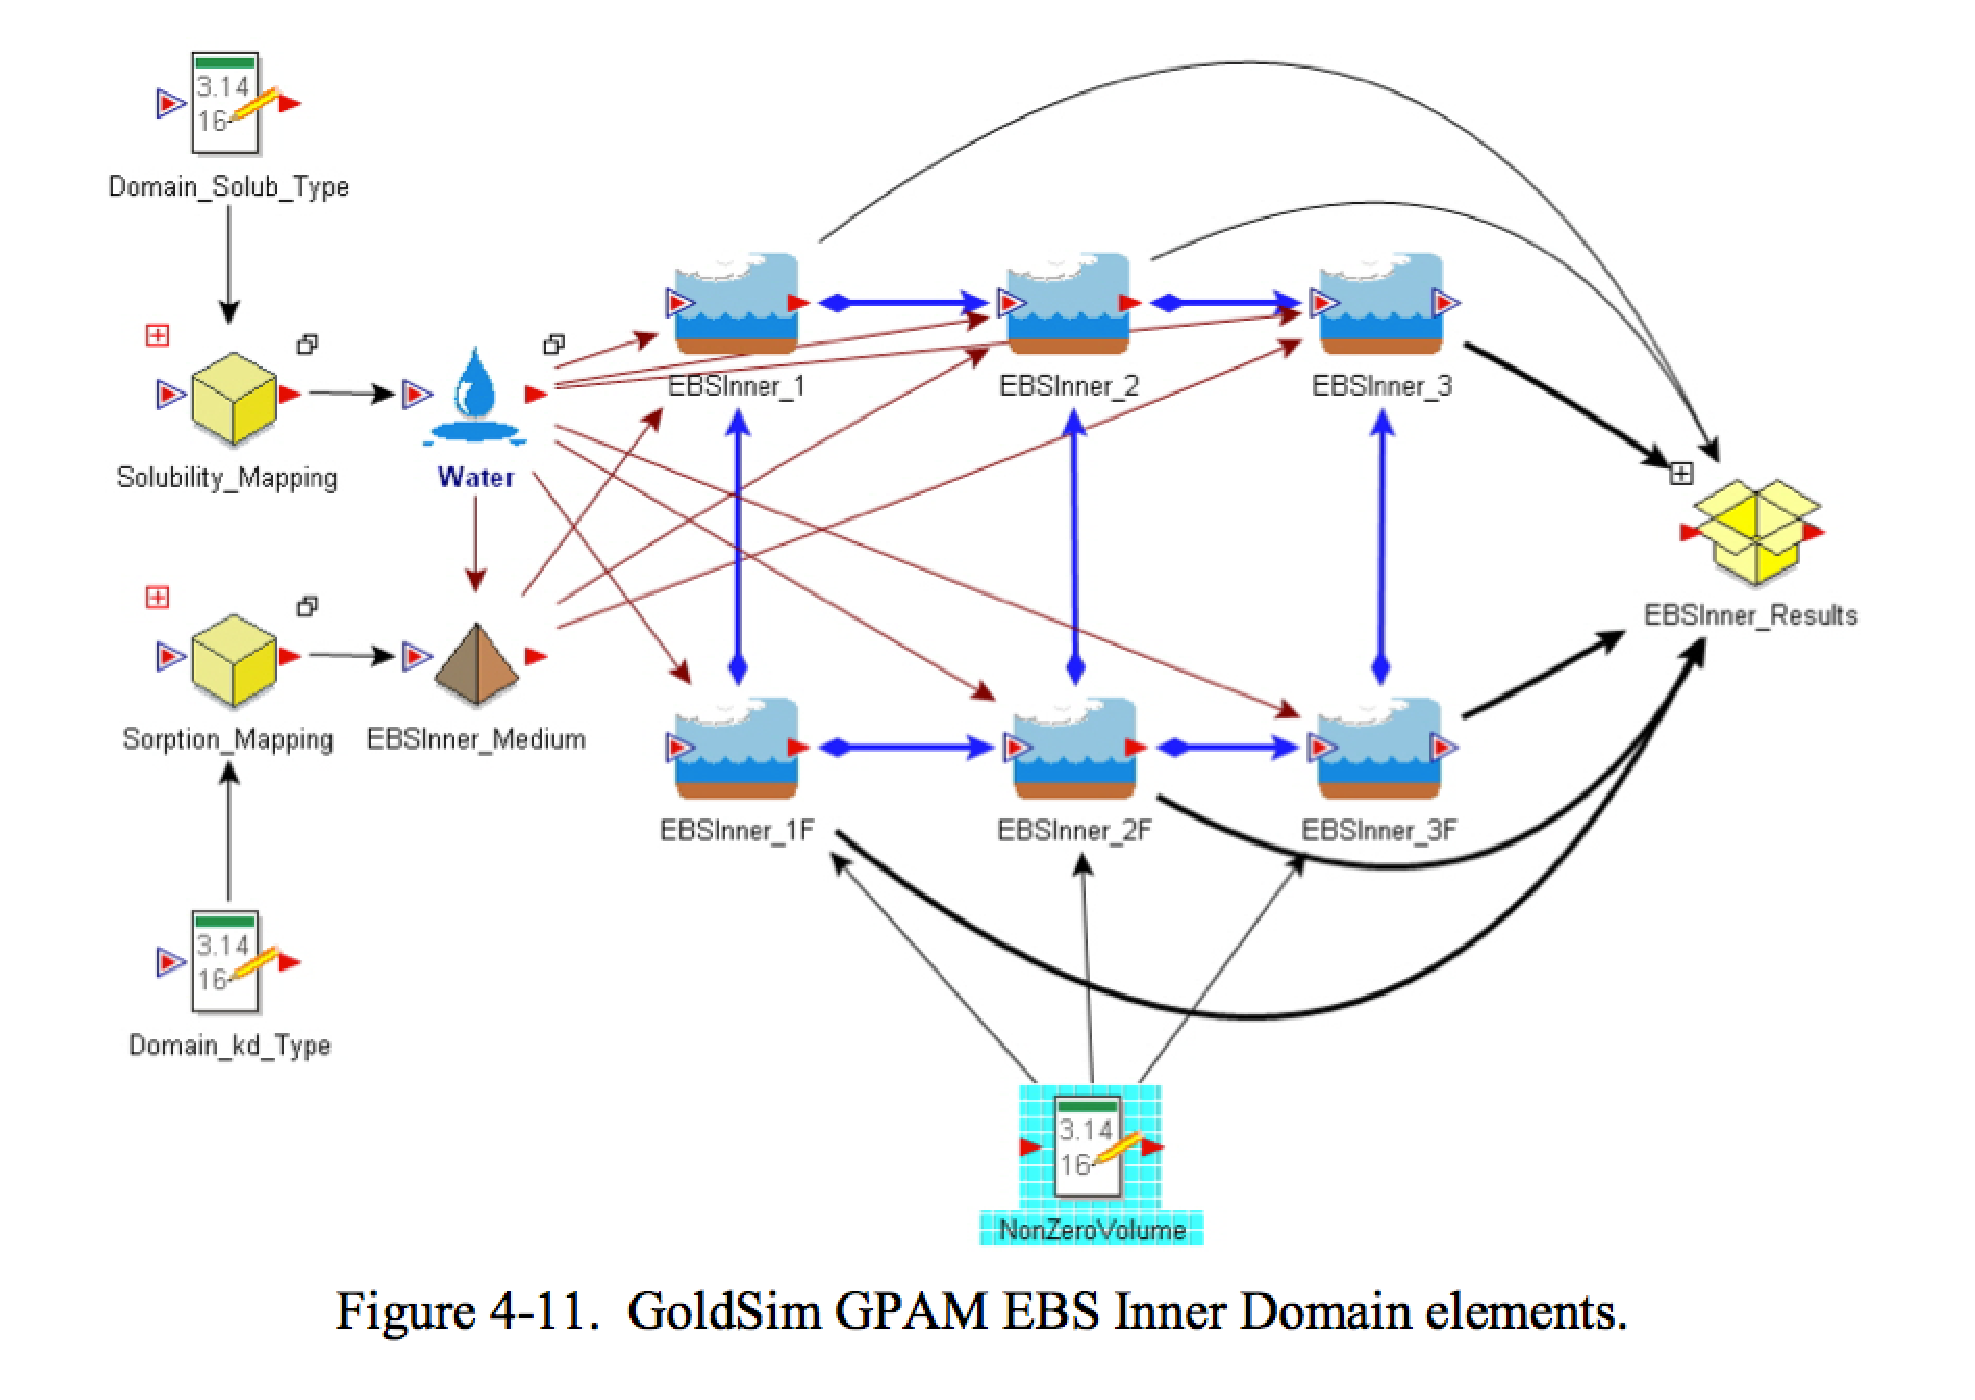
\includegraphics[width=\textwidth]{./images/buffer.eps}
      \end{center}
    \end{figure}
  \end{minipage}
  \hspace{0.01cm}\large{$\rightarrow$}\hspace{0.01cm}
  \begin{minipage}{0.45\textwidth}
    \begin{figure}[h!]
      \begin{center}
        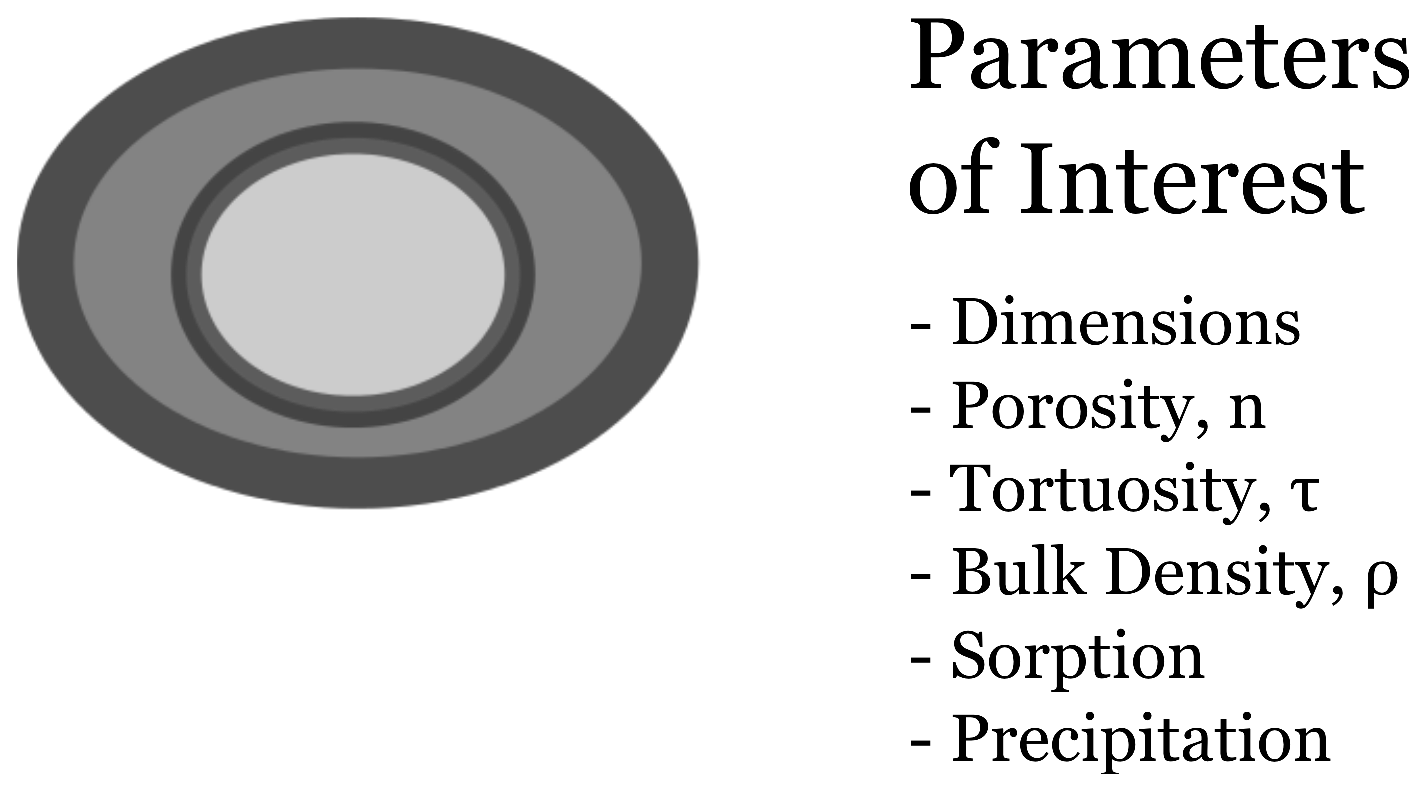
\includegraphics[width=\textwidth]{./images/abstractionBuffer.eps}
      \end{center}
    \end{figure}
  \end{minipage}
\end{frame}

\begin{frame}[ctb!]
  \frametitle{Base Case : Geology Abstraction}
  \begin{minipage}{0.45\textwidth}
    \begin{figure}[h!]
      \begin{center}
        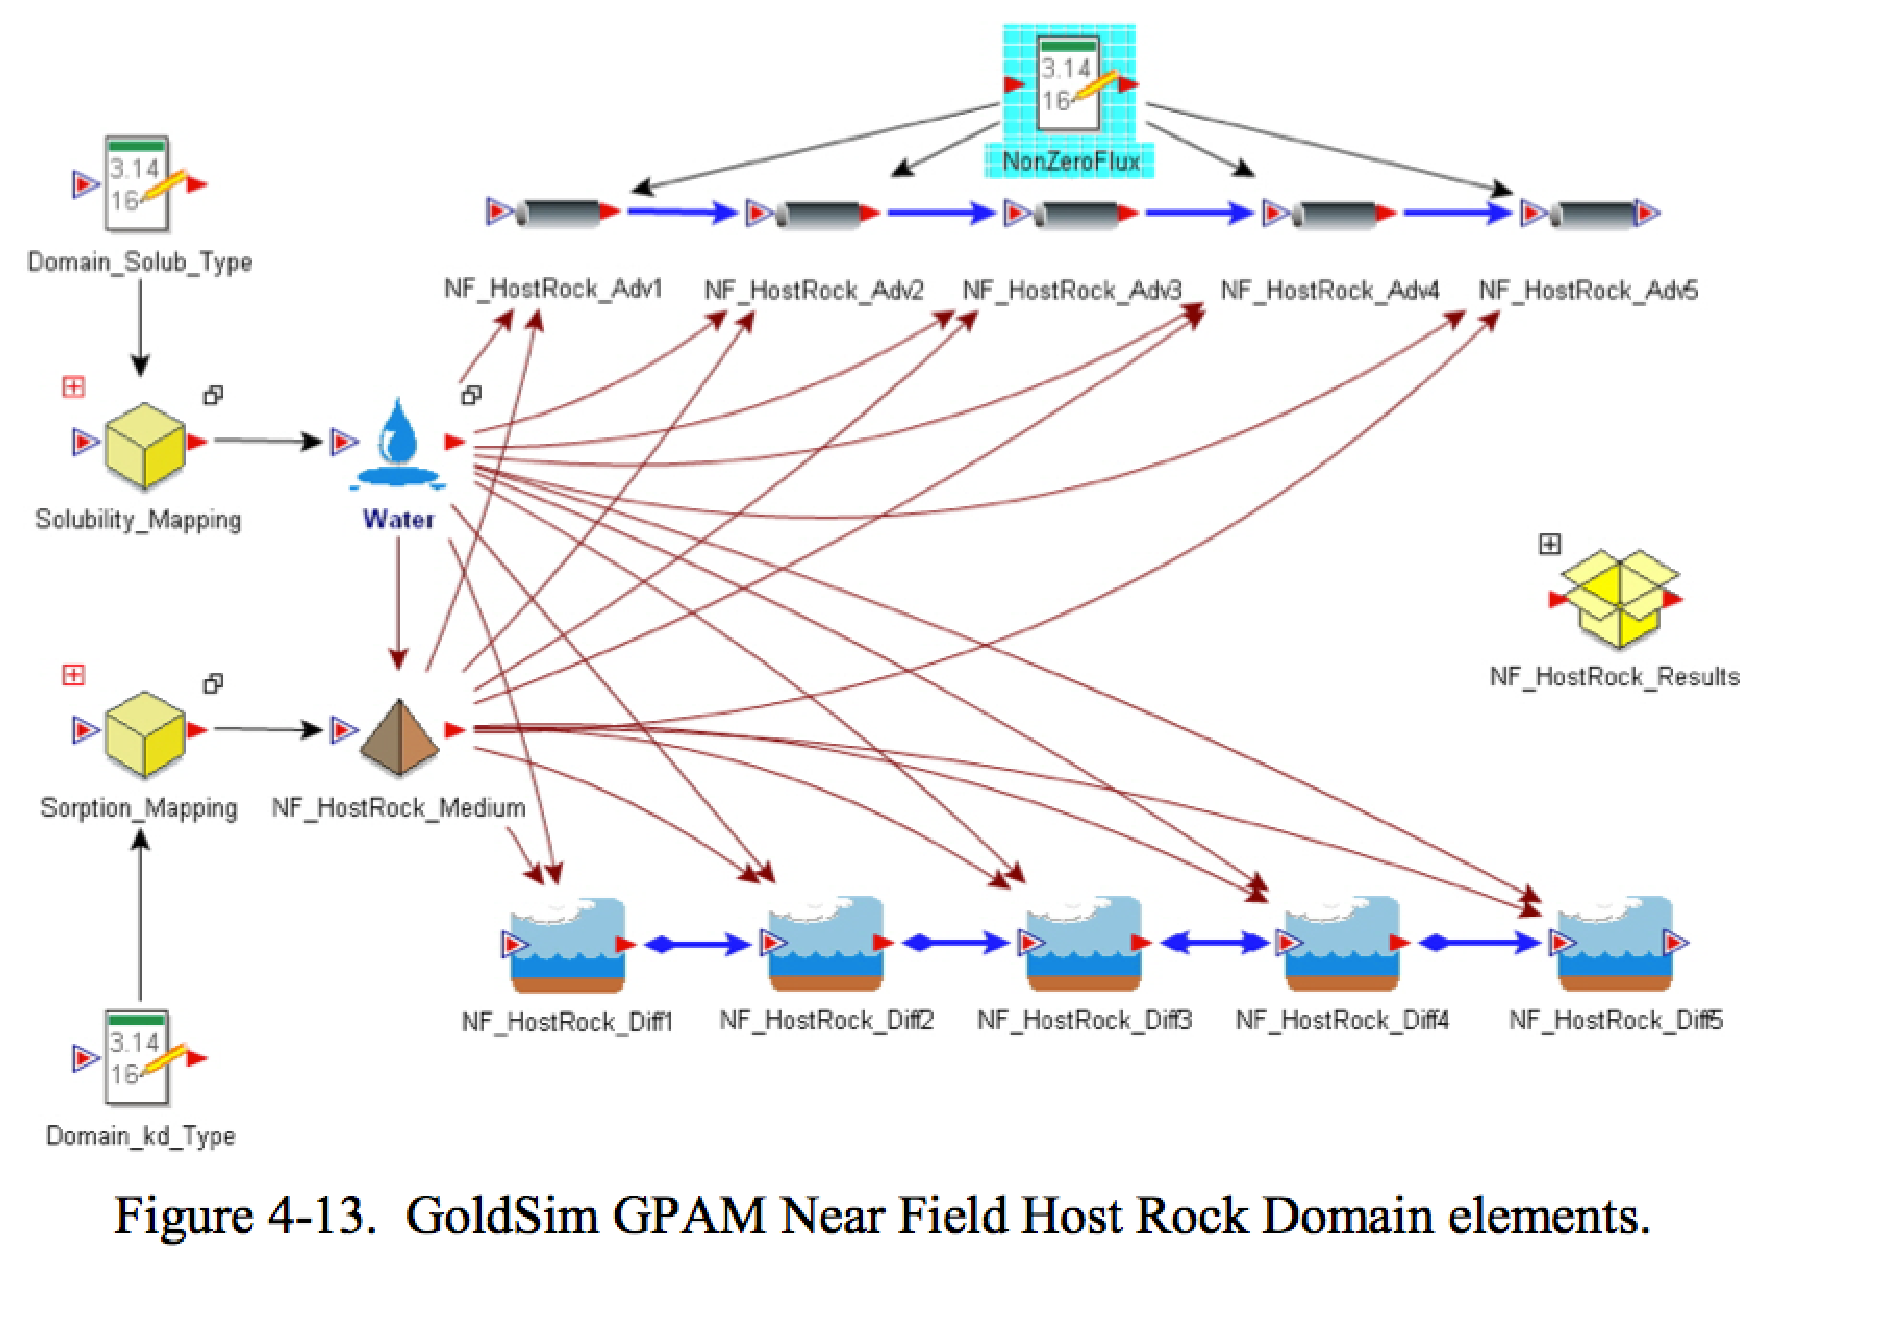
\includegraphics[width=\textwidth]{./images/rock.eps}
      \end{center}
    \end{figure}
  \end{minipage}
  \hspace{0.01cm}\large{$\rightarrow$}\hspace{0.01cm}
  \begin{minipage}{0.45\textwidth}
    \begin{figure}[h!]
      \begin{center}
        \includegraphics[width=\textwidth]{./images/abstractionRock.eps}
      \end{center}
    \end{figure}
  \end{minipage}
\end{frame}

\begin{frame}[ctb!]
  \frametitle{Base Case : System Level Abstraction}
  \begin{figure}[h!]
      \includegraphics[width=\textwidth]{./images/abstractionSystem.eps}
    \caption{System level abstraction seeks to determine the systems level 
    response to the change in models of subcomponents.}
  \end{figure}
\end{frame}

\subsection{Sensitivity Studies}
\begin{frame}[ctb]
\frametitle{Solubility Sensitivity}
\begin{figure}[ht]
  \centering
  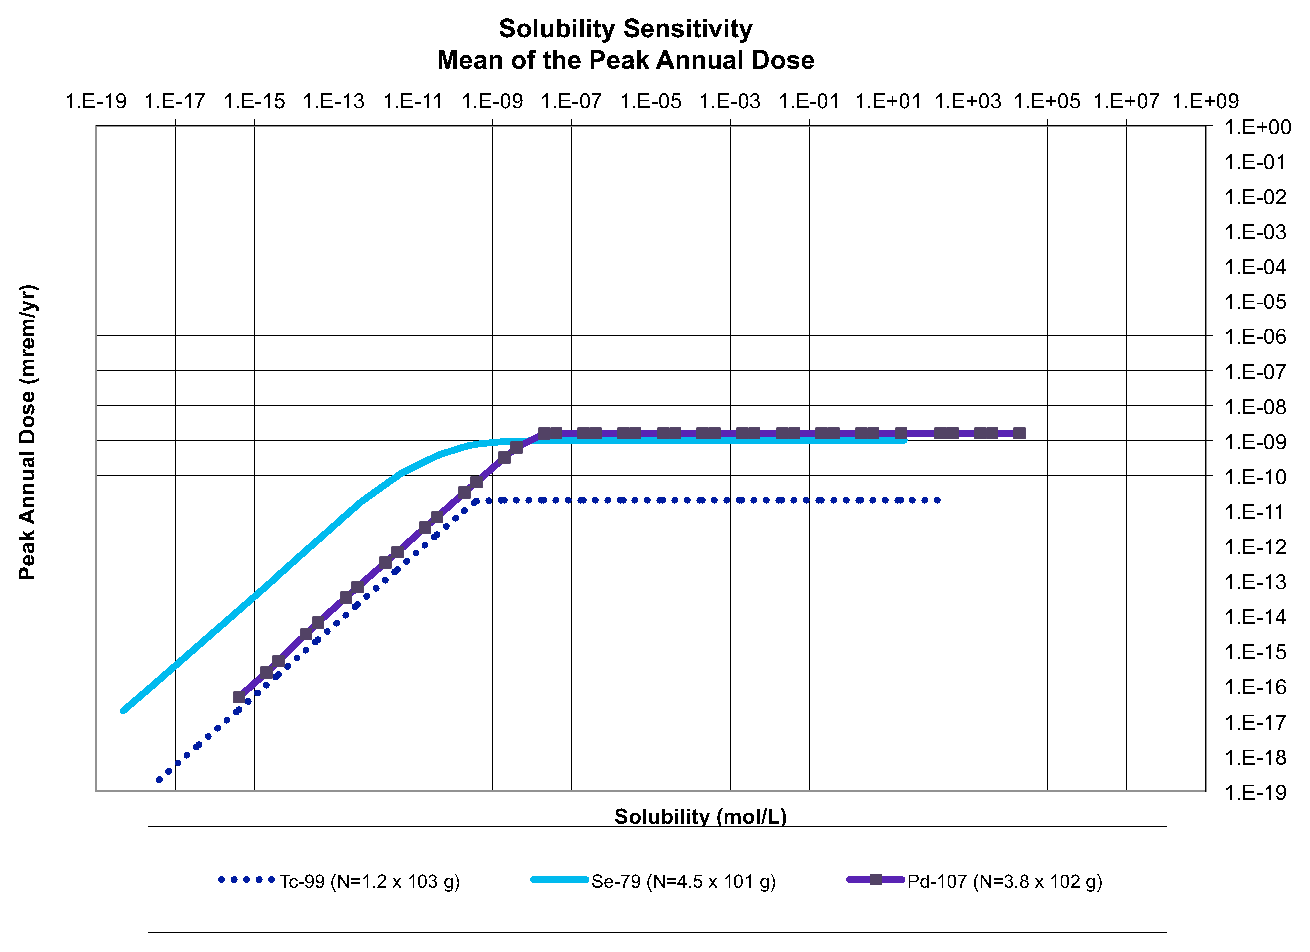
\includegraphics[width=\linewidth]{Solubility_Summary.eps}
  \caption{Solubility limit sensitivity. The peak annual dose due to an 
  inventory, 
  $N$, of each isotope.}
  \label{fig:SolSum}
\end{figure}
\end{frame}

\begin{frame}[ctb]
\frametitle{Retardation Sensitivity}
\begin{figure}[ht]
  \centering
  \includegraphics[width=\linewidth]{Partitioning_Summary.eps}
  \caption{$K_d$ sensitivity.  The peak annual dose due to an inventory, 
  $N$, of each isotope.}
  \label{fig:KdSum}
\end{figure}
\end{frame}



\subsection{Summary}


\begin{frame}[ctb!]
  \frametitle{Integrated Used Fuel Disposition and Repository Model}
  %goal
  %method
  %milestones
\end{frame}




%||||---------------
\begin{frame}[allowframebreaks]
  \frametitle{References}
  \bibliographystyle{plain}
  {\footnotesize \bibliography{prelim}}
\end{frame}
%---------------||||




\end{document}

%\begin{frame}[ctb!]
%  \frametitle{Openness}
%  Openness ensures transparency and lowers institutional technical 
%  obstacles to collaboration.
%\end{frame}


